%% --------------------------------------------------------------------
%% Template UTEC Tesis
%% --------------------------------------------------------------------
% Este es el archivo que se debe compilar.
% 
% Este template ha sido modificado y actualizado por Eduardo Castro y Roosevelt Ubaldo en base a lo trabajado por Víctor Murray, Oscar Ramos y Juan Carlos Barbaran.
%
% Última actualización: Mayo, 2022

\documentclass[a4paper,12pt,oneside]{tesisutec}

\selectlanguage{spanish}

%% Paquetes
\usepackage[utf8]{inputenc}
\usepackage[square, numbers, comma, sort&compress]{natbib}
% Libreria de idioma
\usepackage[spanish]{babel}
% Libreria para posicionamiento
\usepackage{float}
% Librerias para insertar codigos
\usepackage[spanish,onelanguage,ruled,vlined]{algorithm2e}
\usepackage{verbatim} 
% Librería para hipervínculos
\usepackage{hyperref}
% Librería necesaria para arreglar el orden de referencias en overleaf.com
\usepackage{notoccite}
\usepackage{pifont}
\DeclareRobustCommand{\cmark}{\ding{51}}
\DeclareRobustCommand{\xmark}{\ding{55}}

% Incluir acá los paquetes adicionales que deseas. 
\usepackage{tikz}
\usetikzlibrary{arrows.meta,positioning,calc,fit,backgrounds,shapes,babel}

% Ubicación de los imágenes.
\graphicspath{images/}

\makeatletter
% Reinsert missing \algbackskip
\def\algbackskip{\hskip-\ALG@thistlm}
\makeatother

\hypersetup{urlcolor=blue, colorlinks=true}

\begin{document}

\frontmatter

\department{\MakeUppercase{Ciencia de la Computación}}
\degree{Licenciado }
\major{Ciencia de la Computación}

\title{\MakeUppercase{DARL: Aprendizaje por Refuerzo con Diagnóstico de Drift para la Actualización Selectiva de Pipelines Tabulares de ML de Dos Etapas}}

\author{Jeffrey Antonio Monja Castro \orcid{0000-0000-0000-0000}} % Es obligatorio agregar ORCID del alumno
\supervisor{Ariana Mirella Villegas Suárez \orcid{0000-0000-0000-0000}} % Es obligatorio agregar ORCID del asesor

\date{2026}

\maketitle

\setstretch{1.5}


%% ============================================================================
%  Dedicatoria
%% ============================================================================

\dedicatory{Lorem ipsun dolor sit amet}

\input{encabezados/agradecimientos}

\tableofcontents

\newpage

\listoftables

\newpage

\listoffigures

\addtocontents{toc}{\vspace{1.5em}}

%% ============================================================================
\mainmatter
\pagestyle{fancy}

\customchapter{RESUMEN}

Lorem ipsum dolor sit amet.


\noindent \textbf{Palabras clave:}\\
\noindent Palabra clave 1; Palabra clave 2; Palabra clave 3; Palabra clave 4
\customchapter{ABSTRACT} 

\begin{center}
\large \vspace{-1.5cm} \textbf{\MakeUppercase{DARL: Drift-Aware Reinforcement Learning for Selective Updating of Two-Stage Tabular ML Pipelines}}
\end{center}

Lorem ipsum dolor sit amet.


\noindent \textbf{Keywords:}\\
\noindent Keyword 1; Keyword 2; Keyword 3; Keyword 4



\customchapter{INTRODUCCIÓN} 

\introsection{Presentación del tema de investigación}

Los modelos de aprendizaje automático ---o \textit{Machine Learning} (ML)--- desplegados
en producción operan bajo la suposición implícita de que la distribución de los datos de
entrada permanece estable a lo largo del tiempo. Sin embargo, en entornos reales esta
suposición rara vez se sostiene: los patrones demográficos evolucionan, los comportamientos
de los usuarios cambian y los contextos operativos se transforman de manera continua
\cite{mahadevan2024cost}. Cuando la distribución de los datos se aleja de la distribución de
entrenamiento, el rendimiento del modelo se degrada de forma silenciosa pero sistemática,
un fenómeno conocido como \textit{distribution shift} o desplazamiento de la distribución.
 
En \textit{pipelines} de ML de dos etapas ---compuestos por una etapa de \textit{feature
engineering} y una etapa de selección y entrenamiento del modelo predictivo--- esta
degradación puede originarse en cualquiera de las dos etapas o en ambas simultáneamente.
La etapa de preprocesamiento aprende estadísticas de la distribución de entrenamiento:
medias, desviaciones estándar, rangos de valores y frecuencias de categorías. Si la
distribución de los datos de entrada cambia (\textit{covariate shift}), estas estadísticas
quedan desactualizadas y el modelo recibe representaciones distorsionadas de los datos
reales. Por otro lado, si la relación entre las variables de entrada y la variable objetivo
cambia (\textit{concept drift}), el modelo predictivo habrá aprendido reglas que ya no
describen el mundo correctamente, independientemente de lo bien que el preprocesamiento
transforme los datos \cite{cai2023disde}.
 
La respuesta convencional ante la degradación del rendimiento es el reentrenamiento
completo del \textit{pipeline}, que resulta costoso en términos computacionales y
operativos \cite{mahadevan2024cost}. Esta práctica ignora una distinción fundamental: si el
origen del problema es únicamente la etapa de preprocesamiento, actualizar solo esa etapa
podría recuperar el rendimiento a una fracción del costo del reentrenamiento completo. De
manera análoga, si el problema radica en el modelo predictivo, reentrenar únicamente esa
etapa puede ser suficiente. La pregunta de cuándo cada estrategia de actualización selectiva
es suficiente, y a qué costo, no ha sido respondida de forma sistemática en la literatura
existente.
 
Resolver este problema requiere no solo diagnosticar el tipo y la severidad del drift
observado, sino también aprender una política de decisión que, ante un nuevo escenario de
degradación, seleccione la acción más eficiente. Esta investigación propone DARL
(\textit{Drift-Aware Reinforcement Learner}), un framework que formaliza esa política como
un agente de aprendizaje por refuerzo entrenado sobre un Proceso de Decisión de Markov
Parcialmente Observable (POMDP), donde el agente aprende a partir de la experiencia
acumulada sobre múltiples episodios de drift qué acción de actualización maximiza la
recuperación del rendimiento al menor costo computacional.


\introsection{Descripción de la situación problemática}

Los \textit{pipelines} de ML sobre datos tabulares se emplean de manera extensa en
dominios críticos como la salud, las finanzas y las políticas públicas \cite{gardner2023tableshift}.
En estos contextos, la degradación del rendimiento del modelo tiene consecuencias directas
sobre la calidad de las decisiones: un modelo de predicción de mortalidad hospitalaria que
se deteriora silenciosamente puede comprometer la asignación de recursos clínicos, y un
modelo de predicción de ingresos sesgado por cambios demográficos puede distorsionar
políticas de asistencia social.
 
La literatura reciente ha avanzado en el diagnóstico del tipo de drift que afecta a un
modelo \cite{cai2023disde,singh2025shift}, en el estudio de la robustez de distintos modelos frente a
\textit{distribution shift} en \textit{benchmarks} tabulares \cite{gardner2023tableshift} y en la
decisión de cuándo reentrenar considerando el costo computacional \cite{mahadevan2024cost,
shakhovska2025severity}. Sin embargo, estos trabajos presentan una limitación compartida: tratan el
modelo como una unidad indivisible y no estudian la posibilidad de actualizar selectivamente
solo una de las dos etapas del \textit{pipeline}.
 
Esta brecha tiene consecuencias prácticas importantes. En producción, los equipos de
\textit{Data Science} enfrentan la decisión de qué actualizar ante una caída de rendimiento
detectada, sin disponer de un mecanismo que aprenda de manera sistemática cuál es la acción
óptima en función del tipo y la severidad de la deriva observada. La ausencia de una
política de decisión aprendida ---que mapee el estado de las distribuciones observadas a la
acción de actualización más eficiente--- obliga a tomar decisiones \textit{ad hoc},
frecuentemente costosas e innecesarias.


\introsection{Formulación del problema}

La degradación del rendimiento de \textit{pipelines} de ML de dos etapas bajo
\textit{distribution shift} puede originarse en la etapa de \textit{feature engineering},
en la etapa del modelo predictivo o en ambas simultáneamente. Aunque existen métodos para
diagnosticar el tipo de drift \cite{cai2023disde,singh2025shift} y criterios para decidir cuándo
reentrenar \cite{mahadevan2024cost}, no existe un mecanismo que aprenda de forma sistemática
cuál de las cuatro posibles acciones de actualización ---no hacer nada, actualizar solo el
preprocesamiento, actualizar solo el modelo, o reentrenar el \textit{pipeline} completo---
produce la mejor recuperación del rendimiento al menor costo computacional, en función del
tipo de shift (\textit{covariate shift} o \textit{concept drift}) y su severidad (leve,
moderada o severa) sobre datos tabulares reales.
 
A partir de ello, se plantea la siguiente pregunta de investigación: ¿Es posible aprender
una política de decisión mediante aprendizaje por refuerzo que, a partir de señales de
monitoreo del estado de las distribuciones de un \textit{pipeline} de ML de dos etapas,
seleccione la estrategia de actualización selectiva que maximiza la recuperación del
rendimiento predictivo al menor costo computacional, generalizando a escenarios de drift
no vistos durante el entrenamiento?


\introsection{Objetivos de investigación}

Diseñar, implementar y evaluar empíricamente DARL (\textit{Drift-Aware
Reinforcement Learner}), un framework de actualización selectiva para \textit{pipelines} de
ML de dos etapas sobre datos tabulares que aprende una política de decisión mediante
aprendizaje por refuerzo sobre un POMDP formulado a partir del tipo y la severidad del
\textit{distribution shift} detectado, y que cuantifica la recuperación de rendimiento y el
costo computacional asociado a cada acción de actualización.
 
\section*{Objetivos específicos}
 
\begin{enumerate}
    \item Implementar un módulo de monitoreo que detecte y clasifique el tipo de
    \textit{data drift} ---\textit{covariate shift} y \textit{concept drift}---
    mediante el índice de estabilidad poblacional (PSI), el test de
    Kolmogorov--Smirnov (KS) y el \textit{Classifier Two-Sample Test} (C2ST),
    y que cuantifique su severidad mediante un \textit{severity score} combinado.
    Estas métricas constituyen el vector de observación del agente de aprendizaje
    por refuerzo.
 
    \item Formalizar el problema de decisión de actualización selectiva como un
    Proceso de Decisión de Markov Parcialmente Observable (POMDP), donde el espacio
    de acciones comprende las cuatro estrategias de actualización ---diferir la acción,
    actualizar el preprocesamiento, actualizar el modelo predictivo y reentrenar el
    \textit{pipeline} completo---, y la recompensa combina la recuperación del
    AUC-ROC y el costo computacional relativo de cada acción.
 
    \item Entrenar un agente de aprendizaje por refuerzo mediante el algoritmo
    \textit{Proximal Policy Optimization} (PPO) sobre episodios de drift sintético
    controlado, de modo que aprenda una política óptima $\pi^*$ que maximice la
    recompensa acumulada esperada sobre dos conjuntos de datos del
    \textit{benchmark} TableShift \cite{gardner2023tableshift}: Hospital Readmission
    (\texttt{diabetes\_readmission}) y PhysioNet/sepsis (\texttt{physionet}).
 
    \item Evaluar la política aprendida bajo condiciones de drift sintético de tipo
    y severidad conocidos, midiendo la recuperación del AUC-ROC y el costo
    computacional relativo de cada acción, y comparar su desempeño contra una
    tabla de decisión empírica construida como \textit{baseline}.
\end{enumerate}


\introsection{Justificación}

Desde una perspectiva científica, la literatura sobre \textit{distribution shift} en
aprendizaje automático ha avanzado de forma desigual. Los métodos de diagnóstico ---como
DISDE \cite{cai2023disde} y SHIFT \cite{singh2025shift}--- identifican con rigor el tipo de drift que
afecta a un modelo, pero no prescriben ninguna acción correctiva sobre el
\textit{pipeline}. Los métodos de decisión de reentrenamiento ---como CARA
\cite{mahadevan2024cost} y el framework de severidad de Shakhovska y Pukach
\cite{shakhovska2025severity}--- razonan sobre cuándo reentrenar considerando el costo, pero asumen
que el \textit{pipeline} es una unidad monolítica y no distinguen entre sus etapas. Los
trabajos sobre \textit{self-healing pipelines} \cite{tanna2025selfhealing} proponen estrategias de
remediación automática, pero no las evalúan empíricamente en función del tipo de deriva.
Esta investigación cierra ese ciclo al proponer DARL, un framework que conecta el
diagnóstico del drift con una política de decisión aprendida que selecciona la acción
correctiva y cuantifica sus consecuencias sobre el rendimiento y el costo, una contribución
que ninguno de los trabajos previos realiza de forma sistemática.
 
Desde una perspectiva práctica, los equipos de MLOps en producción frecuentemente
reentrenan el \textit{pipeline} completo ante cualquier degradación de rendimiento, sin
evaluar si una actualización parcial sería suficiente. Esta investigación proporciona un
agente entrenado que aprende a tomar decisiones más eficientes, reduciendo el tiempo de
cómputo y los costos operativos en escenarios donde el reentrenamiento selectivo es
suficiente para recuperar el rendimiento. Adicionalmente, el uso de aprendizaje por
refuerzo sobre un dominio de mantenimiento de modelos ---en contraste con su aplicación
habitual en juegos o robótica--- constituye una contribución metodológica con potencial de
generalización a otros problemas de gestión de \textit{pipelines} en producción.


\introsection{Alcance}

La investigación se circunscribe a \textit{pipelines} de ML de dos etapas 
(preprocesamiento y modelo predictivo) aplicados a tareas de clasificación binaria sobre
datos tabulares en modalidad \textit{batch}. La evaluación empírica se realiza sobre dos
conjuntos de datos del \textit{benchmark} TableShift: Hospital Readmission
(\texttt{diabetes\_readmission}) y PhysioNet/sepsis (\texttt{physionet})
\cite{gardner2023tableshift}. El \textit{distribution shift} se
inyecta de forma sintética y controlada en tres niveles de severidad (leve, moderada y
severa) para los tipos \textit{covariate shift}, \textit{concept drift} y su combinación.
El modelo predictivo empleado en los experimentos es XGBoost, con regresión logística como
línea base. El preprocesamiento sigue el esquema de la API de TableShift, extendido con
transformaciones de cuantiles para variables con distribución sesgada y codificación por
objetivo para variables categóricas de alta cardinalidad.
 
El agente de aprendizaje por refuerzo se plantea para entrenamiento mediante PPO,
con un entorno de simulación construido bajo una interfaz compatible con Gymnasium.
El entrenamiento se realiza exclusivamente sobre episodios
de drift sintético generados a partir de los dos datasets seleccionados; no se contempla
despliegue en entornos de producción en tiempo real ni integración con sistemas de
orquestación como Airflow o MLflow.


\introsection{Limitaciones y restricciones}

El framework DARL está orientado a uso académico y experimental. Los experimentos se ejecutan en
modalidad \textit{batch} y no cubren escenarios de \textit{streaming} con drift gradual y
continuo. La evaluación se restringe a los dos \textit{datasets} seleccionados y a un
modelo predictivo principal; la generalización de los resultados a otros dominios y
arquitecturas requiere validación adicional. Asimismo, se asume disponibilidad de etiquetas
en el conjunto de datos del dominio objetivo para realizar el reentrenamiento, condición que
en escenarios reales puede requerir anotación humana o mecanismos de \textit{delayed
feedback}. La política aprendida por el agente PPO está condicionada a la distribución de
episodios de entrenamiento generados; su transferencia a dominios con características de
drift muy distintas a las del entrenamiento requiere fine-tuning o reentrenamiento del
agente. Finalmente, el estudio no evalúa estrategias de defensa ante drift ni métodos de
reentrenamiento incremental, que se consideran líneas de trabajo futuro.

\chapter{REVISIÓN CRÍTICA DE LA LITERATURA}
 
La literatura sobre el mantenimiento de modelos de aprendizaje automático bajo
\textit{distribution shift} se ha desarrollado a lo largo de cuatro líneas relativamente
independientes: el diagnóstico del tipo de drift, la evaluación de la robustez de modelos
tabulares, la decisión de cuándo reentrenar y la automatización de la remediación en
\textit{pipelines} de producción. Aunque cada una de estas líneas ha producido
contribuciones valiosas, ninguna ha abordado de forma conjunta la pregunta de qué etapa de
un \textit{pipeline} de dos etapas conviene actualizar, cuánto se recupera el rendimiento
con cada acción y a qué costo computacional, en función del tipo y la severidad de drift
detectado, ni ha propuesto aprender esa política de decisión de manera automática mediante
aprendizaje por refuerzo. A continuación se revisa cada línea y se identifican sus
limitaciones frente al problema planteado en esta investigación.
 
\section{Diagnóstico del tipo de distribution shift}
 
Una primera familia de métodos se centra en identificar el tipo de drift que ha afectado a
un modelo sin prescribir ninguna acción correctiva sobre el \textit{pipeline}. Cai et
al.~\cite{cai2023disde} proponen DISDE (\textit{DIstribution Shift DEcomposition}), un framework
que descompone la caída de rendimiento de un modelo en dos términos: uno atribuible a
cambios en la distribución marginal de las variables de entrada $P(X)$ (\textit{covariate
shift}) y otro atribuible a cambios en la relación condicional $P(Y \mid X)$
(\textit{concept drift}). La descomposición se construye sobre una distribución compartida
entre los dominios de entrenamiento y destino, lo que permite cuantificar la contribución
de cada tipo de cambio al deterioro observado. DISDE valida su método sobre el
\textit{dataset} Adult Census con modelos de Random Forest de profundidad restringida, lo
que limita deliberadamente la complejidad del clasificador para hacer más observable la
atribución del deterioro a cada tipo de drift.
 
A pesar de su rigor, DISDE presenta dos limitaciones relevantes para esta investigación.
En primer lugar, el método se detiene en el diagnóstico: no especifica qué componente del
\textit{pipeline} debe actualizarse en respuesta a la descomposición obtenida, ni evalúa si
distintas acciones correctivas producen recuperaciones de rendimiento diferentes. En segundo
lugar, DISDE no estudia cómo la magnitud de drift ---su severidad--- modifica la relación
entre el tipo diagnosticado y la acción más conveniente. Desde la perspectiva del POMDP
propuesto en esta investigación, DISDE aporta evidencia sobre la señal de diagnóstico pero
no sobre la política de acción.
 
Singh et al.~\cite{singh2025shift} proponen SHIFT (\textit{Subgroup-scanning Hierarchical
Inference Framework for performance drifT}), un framework no paramétrico de dos etapas que
primero detecta si algún subgrupo de la población experimenta una caída de rendimiento
inaceptable debido a \textit{covariate shift} o \textit{outcome shift} agregados, y luego
identifica los subconjuntos de variables responsables. A diferencia de DISDE, SHIFT aborda
el diagnóstico mediante pruebas de hipótesis en lugar de estimación, lo que le permite
operar con conjuntos de datos más pequeños sin asumir modelos paramétricos ni el grafo
causal entre variables. En un experimento real sobre predicción de readmisión hospitalaria,
SHIFT guía una corrección dirigida al modelo y demuestra que esta supera al reentrenamiento
no dirigido.
 
No obstante, SHIFT presenta limitaciones similares a las de DISDE desde la perspectiva de
esta investigación. El framework trata el modelo predictivo como una unidad monolítica y no
considera la posibilidad de actualizar únicamente la etapa de preprocesamiento. Tampoco
evalúa sistemáticamente cómo la severidad de drift modifica la relación entre el diagnóstico
y la acción óptima, ni mide el costo computacional de las distintas correcciones. En
términos del POMDP, SHIFT enriquece la señal de observación (señala subgrupos afectados),
pero no resuelve el problema de aprendizaje de la política de decisión.
 
\section{Benchmarking de robustez ante distribution shift en datos tabulares}
 
Una segunda línea de investigación aborda la ausencia de \textit{benchmarks} estandarizados
para evaluar la robustez de modelos de clasificación tabular ante drift de distribución
real. Gardner et al.~\cite{gardner2023tableshift} introducen TableShift, un \textit{benchmark} que
comprende 15 tareas de clasificación binaria sobre dominios de finanzas, salud, educación y
política pública, cada una acompañada de una partición de dominio que induce una brecha de
rendimiento estadísticamente significativa entre los datos de entrenamiento y los datos fuera
de distribución. Su estudio a gran escala ---que evalúa 18 modelos, incluyendo XGBoost,
LightGBM, redes neuronales profundas y transformadores tabulares--- revela una tendencia
lineal entre la precisión en distribución y fuera de distribución, y muestra que ningún
modelo ni método de robustez de dominio cierra consistentemente la brecha de rendimiento.
 
Desde una perspectiva metodológica, TableShift ofrece una API Python que proporciona
documentación de tipos de \textit{features}, preprocesamiento estandarizado y particiones de
dominio reproducibles, lo que lo convierte en la fuente de datos natural para los
experimentos de esta investigación y para la generación de episodios de entrenamiento del
agente de aprendizaje por refuerzo. Sin embargo, TableShift evalúa únicamente modelos
estáticos bajo drift real y no experimenta con ninguna estrategia de actualización
post-drift. El \textit{benchmark} caracteriza el problema de drift en datos tabulares sin
proporcionar evidencia sobre la solución de actualización selectiva del \textit{pipeline} ni
sobre la política de decisión óptima.
 
\section{Decisiones de reentrenamiento con conciencia del costo}
 
Una tercera línea estudia cuándo es económicamente justificado reentrenar un modelo tras
detectar drift, considerando explícitamente el trade-off entre el costo de mantener un
modelo desactualizado y el costo del reentrenamiento. Mahadevan y
Mathioudakis~\cite{mahadevan2024cost} formulan este problema como una decisión de optimización
y proponen CARA (\textit{Cost-Aware Retraining Algorithm}), que toma decisiones de
reentrenamiento sobre flujos de datos y consultas minimizando el costo total esperado. Sus
experimentos sobre \textit{datasets} sintéticos y reales demuestran que CARA realiza menos
decisiones de reentrenamiento que los \textit{baselines} basados en detección de drift,
incurriendo en menores costos totales. Este trabajo introduce la dimensión de costo
computacional que esta investigación retoma, pero opera sobre un modelo de una sola etapa
y es agnóstico al tipo de drift: toma sus decisiones en función de la degradación de
rendimiento agregada sin distinguir si esta proviene de \textit{covariate shift} o de
\textit{concept drift}. Además, CARA emplea reglas determinísticas basadas en umbrales,
mientras que esta investigación propone una política aprendida mediante aprendizaje por
refuerzo que puede adaptarse a combinaciones de señales no vistas.
 
Shakhovska y Pukach~\cite{shakhovska2025severity} extienden esta perspectiva introduciendo un
\textit{severity score} como señal para calibrar la intensidad de la respuesta. El score
combina la estadística de Kolmogorov--Smirnov, la distancia de Wasserstein y la divergencia
de Jensen--Shannon en una métrica ponderada que alimenta una política de tres niveles: el
drift menor se ignora, la moderada dispara actualizaciones incrementales del modelo y la
severa inicia el reentrenamiento completo. Los autores reportan reducciones en el cómputo
innecesario y reconocen explícitamente como trabajo futuro la necesidad de ``adaptar no solo
a la severidad sino también al tipo de drift'' para habilitar actualizaciones más precisas y
contextualizadas. Al igual que CARA, este framework trata el sistema de aprendizaje
automático como una unidad indivisible y no evalúa la posibilidad de actualizar únicamente
la etapa de preprocesamiento. Su política de tres niveles es fija y no se adapta a nuevos
patrones de drift sin rediseño manual, limitación que el enfoque de aprendizaje por refuerzo
propuesto en esta investigación supera de forma directa.
 
\section{Self-healing pipelines y automatización de la remediación}
 
Una cuarta línea sistematiza las estrategias de remediación automática en \textit{pipelines}
de ML en producción. Tanna~\cite{tanna2025selfhealing} presenta una revisión comprensiva de los
patrones arquitectónicos, los mecanismos de detección y las estrategias de remediación
---incluyendo reentrenamiento incremental, \textit{rollback} a modelos estables, cambio de
\textit{ensemble} y actualización activa--- con casos de estudio en detección de fraude
financiero, predicción de riesgo clínico y sistemas de recomendación en comercio
electrónico. El trabajo concluye que la elección de la estrategia de remediación depende
del trade-off entre latencia, precisión y costo operativo, y proporciona orientación
cualitativa para diseñadores de sistemas de producción. Notablemente, el propio survey
señala como dirección futura la integración con aprendizaje por refuerzo para mecanismos de
remediación más adaptativos, anticipando el enfoque que esta investigación desarrolla.
 
Sin embargo, este trabajo no conduce experimentos controlados que midan cuánto rendimiento
recupera cada estrategia en función del tipo o la severidad de drift, y no diferencia entre
actualizar etapas individuales del \textit{pipeline} versus reentrenar el sistema completo.
El survey ofrece orientación operativa sin la evidencia cuantitativa necesaria para
prescribir cuál acción es óptima bajo qué condiciones, ni proporciona un mecanismo que
aprenda esa correspondencia de manera automática.
 
\section{Síntesis y brecha identificada}
 
La Tabla~\ref{tab:comparacion} resume las dimensiones abordadas por cada trabajo relacionado
y contrasta con las contribuciones de la presente investigación.
 
\begin{table}[h]
\centering
\caption{Comparación de trabajos relacionados}
\label{tab:comparacion}
\resizebox{0.98\textwidth}{!}{%
\begin{tabular}{lcccccc}
\hline
\textbf{Trabajo} &
\textbf{\begin{tabular}[c]{@{}c@{}}Diagnóstico\\tipo drift\end{tabular}} &
\textbf{\begin{tabular}[c]{@{}c@{}}Niveles de\\severidad\end{tabular}} &
\textbf{\begin{tabular}[c]{@{}c@{}}Pipeline\\dos etapas\end{tabular}} &
\textbf{\begin{tabular}[c]{@{}c@{}}Recuperación\\medida\end{tabular}} &
\textbf{\begin{tabular}[c]{@{}c@{}}Costo\\cómputo\end{tabular}} &
\textbf{\begin{tabular}[c]{@{}c@{}}Política\\aprendida (RL)\end{tabular}} \\
\hline
DISDE \cite{cai2023disde}           & \checkmark & $\times$ & $\times$ & $\times$ & $\times$ & $\times$ \\
SHIFT \cite{singh2025shift}         & \checkmark & $\times$ & $\times$ & \checkmark & $\times$ & $\times$ \\
TableShift \cite{gardner2023tableshift}  & $\times$   & $\times$ & $\times$ & $\times$ & $\times$ & $\times$ \\
CARA \cite{mahadevan2024cost}      & $\times$   & $\times$ & $\times$ & \checkmark & \checkmark & $\times$ \\
Severity-Aware \cite{shakhovska2025severity} & $\times$ & \checkmark & $\times$ & \checkmark & \checkmark & $\times$ \\
Self-Healing \cite{tanna2025selfhealing}  & $\times$   & $\times$ & $\times$ & $\times$ & \checkmark & $\times$ \\
\textbf{DARL}    & \checkmark & \checkmark & \checkmark & \checkmark & \checkmark & \checkmark \\
\hline
\end{tabular}%
}
\begin{flushleft}
\footnotesize\textit{Nota.} \checkmark~= abordado; $\times$~= no abordado.
\end{flushleft}
\end{table}

 
La tabla revela una brecha consistente: ningún trabajo existente aborda simultáneamente (a)
el diagnóstico del tipo y la severidad de drift, (b) la distinción entre etapas de un
\textit{pipeline} de dos etapas como unidades de actualización independientes, (c) la
medición cuantitativa de la recuperación de rendimiento y el costo computacional de cada
acción, y (d) el aprendizaje automático de una política de decisión mediante aprendizaje
por refuerzo que generalice a escenarios de drift no vistos.
 
Los métodos de diagnóstico (DISDE, SHIFT) establecen con rigor qué tipo de drift ha
ocurrido, pero dejan sin responder qué acción tomar. Los métodos de decisión de
reentrenamiento (CARA, Severity-Aware) razonan sobre cuándo actuar y a qué costo, pero
asumen que el \textit{pipeline} es una sola pieza, son agnósticos al tipo de drift y
emplean políticas de umbral fijo no adaptativas. Los trabajos de \textit{benchmarking}
(TableShift) caracterizan el problema sin proponer soluciones de adaptación. Los surveys de
\textit{self-healing} (Tanna) organizan el espacio de estrategias sin evaluarlas
empíricamente y sin proponer un mecanismo de aprendizaje.
 
Esta investigación aborda esa brecha al proponer DARL, un framework que (a) usa herramientas
estándar de detección de drift ---PSI, KS y C2ST--- para construir el vector de observación
del agente, (b) formaliza el problema de decisión como un POMDP donde el agente aprende
mediante PPO a seleccionar la acción de actualización óptima entre cuatro posibles, y (c)
mide la recuperación de AUC-ROC y el costo computacional relativo de la política aprendida
bajo condiciones de drift sintético controlado sobre \textit{benchmarks} tabulares reales,
comparándola contra una tabla de decisión empírica construida como \textit{baseline}. El
resultado es un agente DARL que internaliza el trade-off rendimiento--costo y generaliza a
combinaciones de tipo y severidad de drift no observadas durante el entrenamiento.
\chapter{MARCO TEÓRICO}

Este capítulo desarrolla los fundamentos conceptuales y formales sobre los que se
construye DARL. La presentación sigue el orden lógico del framework: primero se
describe el dominio de aplicación de la tesis (datos tabulares), luego se formaliza
el objeto de estudio (el \textit{pipeline} de dos etapas), después se introduce el
fenómeno que perturba su funcionamiento (\textit{distribution shift}), posteriormente
se presentan las señales que permiten observarlo (métricas de monitoreo), y
finalmente se desarrolla el formalismo de decisión y el algoritmo de aprendizaje
que constituyen el núcleo de la contribución (POMDP y PPO).

% ------------------------------------------------------------
\section{Datos tabulares en aprendizaje automático}
% ------------------------------------------------------------

Los datos tabulares constituyen una de las formas más comunes de representación de
información estructurada en aplicaciones reales de aprendizaje automático. En este
tipo de datos, cada observación se organiza como una fila de una tabla y cada
variable o atributo se representa como una columna. A diferencia de dominios como
visión por computadora o procesamiento de lenguaje natural, donde las entradas
suelen tener una estructura homogénea, los datos tabulares combinan variables
numéricas, categóricas, ordinales, binarias y valores faltantes dentro de una misma
representación.

Formalmente, un conjunto de datos tabular supervisado puede representarse como:

\begin{equation}
    \mathcal{D} = \{(x_i, y_i)\}_{i=1}^{n}, \qquad
    x_i = (x_{i1}, x_{i2}, \ldots, x_{id}) \in \mathcal{X}.
    \label{eq:tabular_dataset}
\end{equation}

\noindent\textbf{Donde:}
\begin{itemize}
    \item $\mathcal{D}$ representa el conjunto de datos disponible para entrenamiento, validación o evaluación.
    \item $n$ representa el número total de observaciones o filas de la tabla.
    \item $x_i$ representa la observación tabular número $i$.
    \item $y_i$ representa la etiqueta o variable objetivo asociada a la observación $x_i$.
    \item $x_{ij}$ representa el valor de la variable o columna $j$ para la observación $i$.
    \item $d$ representa el número de variables originales en la tabla.
    \item $\mathcal{X}$ representa el espacio de entrada formado por las observaciones tabulares crudas.
\end{itemize}

Conceptualmente, esta notación muestra que una tabla no es solo una matriz de valores,
sino una colección de observaciones con atributos heterogéneos y una variable objetivo.
Esta heterogeneidad es relevante porque distintas columnas requieren tratamientos
diferentes antes de ser usadas por un modelo predictivo. Por ejemplo, las variables
numéricas pueden requerir escalamiento o transformación de cuantiles, mientras que las
variables categóricas pueden requerir codificación, agrupamiento de categorías raras o
manejo explícito de valores desconocidos.

En consecuencia, el desempeño de un modelo tabular no depende únicamente del
algoritmo predictivo, sino también de las decisiones de preprocesamiento aplicadas antes
del entrenamiento. Esta característica distingue a los sistemas tabulares de otros dominios
donde las representaciones suelen aprenderse de manera más integrada. En problemas
tabulares, la etapa de \textit{feature engineering} puede modificar la escala, la dimensión y
la semántica de las variables que recibe el modelo.

TableShift es especialmente relevante para esta investigación porque fue propuesto como
un \textit{benchmark} para estudiar \textit{distribution shift} en tareas de clasificación
binaria con datos tabulares reales \cite{gardner2023tableshift}. Este \textit{benchmark}
reúne tareas de distintos dominios, como salud, finanzas, educación, política pública y
participación cívica, y permite evaluar cómo cambia el desempeño de los modelos cuando
la distribución de prueba difiere de la distribución de entrenamiento. Por ello, TableShift
sirve como referencia conceptual y experimental para estudiar la robustez de modelos
tabulares ante cambios de distribución.

Para DARL, la importancia de los datos tabulares no se limita al tipo de datos utilizado,
sino que define el problema de mantenimiento del \textit{pipeline}. Si cambian las
frecuencias de categorías, los rangos numéricos, la proporción de valores faltantes o las
relaciones entre variables, los parámetros aprendidos por el preprocesamiento pueden
quedar desactualizados. Esto justifica separar explícitamente la etapa de transformación
de características y la etapa predictiva, como se formaliza en la siguiente sección.

% ------------------------------------------------------------
\section{Pipelines de ML de dos etapas sobre datos tabulares}
% ------------------------------------------------------------
 
Un \textit{pipeline} de aprendizaje automático sobre datos tabulares es un sistema
compuesto por una secuencia de operaciones que transforma observaciones crudas en
predicciones. En esta investigación se considera un \textit{pipeline} de dos etapas:
una etapa de \textit{feature engineering} o preprocesamiento, encargada de convertir
los datos tabulares originales en una representación utilizable por el modelo, y una
etapa de modelo predictivo, encargada de aprender la relación entre dicha representación
y la variable objetivo.

Esta separación es importante porque ambos componentes pueden verse afectados de
manera distinta ante cambios de distribución. Un cambio en la distribución marginal de
las variables de entrada puede volver obsoletas las estadísticas aprendidas por el
preprocesamiento, mientras que un cambio en la relación entre entrada y salida puede
volver obsoletos los parámetros del modelo predictivo. Por ello, DARL analiza el
\textit{pipeline} como una composición de dos funciones con parámetros diferentes.
 
La primera etapa, denominada \textit{feature engineering} o preprocesamiento, puede
formalizarse mediante una función parametrizada:

\begin{equation}
    f_\phi: \mathcal{X} \rightarrow \mathcal{Z}.
    \label{eq:feature_engineering_mapping}
\end{equation}

\noindent\textbf{Donde:}
\begin{itemize}
    \item $\mathcal{X} \subseteq \mathbb{R}^{d}$ corresponde al espacio de entrada original, compuesto por los datos tabulares crudos. Se define como un vector de $d$ variables o columnas.
    \item $\mathcal{Z} \subseteq \mathbb{R}^{k}$ representa el espacio transformado o representación intermedia utilizada por el modelo predictivo con $k$ variables, que pueden diferir de las $d$ variables originales.
    \item $f_\phi$ representa la función de preprocesamiento o ingeniería de características.
    \item $\phi$ representa los parámetros asociados a dicha función, tales como medias, desviaciones estándar, codificaciones categóricas, cuantiles o reglas de imputación aprendidas durante el entrenamiento.
\end{itemize}

Conceptualmente, esta notación muestra que la etapa de \textit{feature\ engineering} no es solo una transformación fija, sino un proceso parametrizado que puede modificar la dimensión y la escala de los datos. Esto es especialmente importante en datos tabulares, donde las variables numéricas, categóricas y ordinales requieren tratamientos diferentes antes de ser usadas por un modelo predictivo. Así, herramientas como escaladores, imputadores o codificadores aprenden valores a partir del entrenamiento para transformar nuevos datos; por ello, ante cambios en la distribución de entrada, los parámetros ($\phi$) pueden volverse obsoletos y requerir actualización.
 
La segunda etapa, denominada modelo predictivo, se define como una función que toma
la representación intermedia y produce una salida:

\begin{equation}
    g_\theta: \mathcal{Z} \rightarrow \mathcal{Y}.
    \label{eq:model_mapping}
\end{equation}

\noindent\textbf{Donde:}
\begin{itemize}
    \item $\mathcal{Z} \subseteq \mathbb{R}^{k}$ representa el espacio de características ya transformadas por la etapa de preprocesamiento.
    \item $\mathcal{Y} \subseteq \mathbb{R}$ representa el espacio de salida, como las clases resultantes.
    \item $g_\theta$ representa el modelo predictivo entrenado sobre las características transformadas.
    \item $\theta$ representa los parámetros aprendidos del modelo, como pesos, umbrales, estructuras de árboles o hiperparámetros ajustados durante el entrenamiento.
\end{itemize}

Conceptualmente, esta fórmula separa claramente el rol del preprocesamiento y el rol
del modelo. Mientras $f_\phi$ transforma los datos, $g_\theta$ aprende la relación entre
la representación transformada y la variable objetivo. En esta investigación, el modelo
predictivo principal es XGBoost \cite{chen2016xgboost}, con regresión logística como
línea base.
 
La función de predicción del \textit{pipeline} completo se obtiene componiendo ambas
etapas:

\begin{equation}
    h = g_\theta \circ f_\phi, \qquad
    \hat{y} = h(x) = g_\theta\!\left(f_\phi(x)\right).
    \label{eq:pipeline_composition}
\end{equation}

\noindent\textbf{Donde:}
\begin{itemize}
    \item $h$ representa la función completa del \textit{pipeline} de ML.
    \item $\circ$ representa la composición de funciones, es decir, aplicar primero $f_\phi$ y luego $g_\theta$.
    \item $x$ representa una observación tabular cruda.
    \item $f_\phi(x)$ representa la versión transformada de la observación $x$.
    \item $g_\theta(f_\phi(x))$ representa la predicción producida por el modelo a partir de la observación transformada.
    \item $\hat{y}$ representa la salida predicha por el \textit{pipeline}.
\end{itemize}

Esta composición expresa que la predicción final depende tanto de la
calidad de la transformación como de la calidad del modelo. Si el rendimiento de $h$ se
degrada, el origen del problema puede estar en $f_\phi$, en $g_\theta$ o en ambos. Esta
separación es la base del problema de actualización selectiva que DARL busca resolver:
identificar qué componente debe actualizarse bajo distintos tipos de drift.
 
% ------------------------------------------------------------
\section{Distribution shift: taxonomía y formalización}
% ------------------------------------------------------------
 
Sea $P_{\text{tr}}(X,Y)$ la distribución conjunta de entrada y salida durante el
entrenamiento, y sea $P_{\text{te}}(X,Y)$ la distribución conjunta durante el despliegue.
De forma general, existe \textit{distribution shift} cuando:
 
\begin{equation}
    P_{\text{tr}}(X,Y) \neq P_{\text{te}}(X,Y).
    \label{eq:distribution_shift}
\end{equation}
 
\noindent\textbf{Donde:}
\begin{itemize}
    \item $X$ representa las variables de entrada o características del problema.
    \item $Y$ representa la variable objetivo o etiqueta que se desea predecir.
    \item $P_{\text{tr}}(X,Y)$ representa la distribución conjunta observada durante el entrenamiento.
    \item $P_{\text{te}}(X,Y)$ representa la distribución conjunta observada durante el despliegue o evaluación.
\end{itemize}

Conceptualmente, esta fórmula indica que el modelo fue entrenado bajo una distribución
estadística distinta a la que enfrenta durante producción. Esta diferencia puede hacer que
un modelo con buen desempeño durante entrenamiento pierda precisión en despliegue,
incluso si su arquitectura y sus parámetros no han cambiado \cite{gama2014survey,cai2023disde}.

La distribución conjunta puede factorizarse en una distribución marginal de entrada y
una distribución condicional de salida:

\begin{equation}
    P(X,Y) = P(X)\,P(Y \mid X).
    \label{eq:joint_factorization}
\end{equation}

\noindent\textbf{Donde:}
\begin{itemize}
    \item $P(X,Y)$ representa la distribución conjunta de entradas y salidas.
    \item $P(X)$ representa la distribución marginal de las variables de entrada.
    \item $P(Y \mid X)$ representa la distribución condicional de la variable objetivo dado el valor de las entradas.
\end{itemize}

Conceptualmente, esta descomposición permite distinguir dos fuentes principales de
drift. Puede cambiar la distribución de los datos que llegan al sistema, lo que afecta a
$P(X)$, o puede cambiar la relación entre esos datos y la etiqueta, lo que afecta a
$P(Y \mid X)$. Esta distinción es central porque cada tipo de cambio sugiere una acción
de mantenimiento distinta sobre el \textit{pipeline} \cite{cai2023disde}.
 
\subsection{Covariate shift}
 
El \textit{covariate shift} ocurre cuando cambia la distribución marginal de las variables
de entrada, pero se mantiene estable la relación condicional entre entrada y salida:
 
\begin{equation}
    P_{\text{tr}}(X) \neq P_{\text{te}}(X)
    \quad \text{con} \quad
    P_{\text{tr}}(Y \mid X) = P_{\text{te}}(Y \mid X).
    \label{eq:covariate_shift}
\end{equation}
 
\noindent\textbf{Donde:}
\begin{itemize}
    \item $P_{\text{tr}}(X)$ representa la distribución de las variables de entrada durante el entrenamiento.
    \item $P_{\text{te}}(X)$ representa la distribución de las variables de entrada durante el despliegue.
    \item $P_{\text{tr}}(Y \mid X)$ representa la relación entre entrada y salida aprendida en entrenamiento.
    \item $P_{\text{te}}(Y \mid X)$ representa la relación entre entrada y salida vigente durante el despliegue.
    \item La primera desigualdad indica que los datos de entrada cambiaron.
    \item La igualdad condicional indica que la lógica que relaciona $X$ con $Y$ se mantiene estable.
\end{itemize}

Conceptualmente, el \textit{covariate shift} significa que cambian los datos, pero no
necesariamente cambia la regla del problema. En un \textit{pipeline} de dos etapas, este
tipo de drift afecta directamente al preprocesamiento: los parámetros $\phi$, como medias,
desviaciones estándar, cuantiles o frecuencias categóricas, fueron estimados sobre
$P_{\text{tr}}(X)$ y pueden quedar desactualizados cuando la distribución de entrada cambia.
Por ello, actualizar $f_\phi$ puede ser suficiente si $g_\theta$ todavía representa
adecuadamente la relación $P(Y \mid X)$ \cite{gama2014survey,cai2023disde}.
 
\subsection{Concept drift}
 
El \textit{concept drift} ocurre cuando cambia la relación condicional entre las variables
de entrada y la variable objetivo, incluso si la distribución de entrada permanece estable:
 
\begin{equation}
    P_{\text{tr}}(Y \mid X) \neq P_{\text{te}}(Y \mid X)
    \quad \text{con} \quad
    P_{\text{tr}}(X) = P_{\text{te}}(X).
    \label{eq:concept_drift}
\end{equation}
 
\noindent\textbf{Donde:}
\begin{itemize}
    \item $P_{\text{tr}}(Y \mid X)$ representa la relación entrada-salida observada durante el entrenamiento.
    \item $P_{\text{te}}(Y \mid X)$ representa la relación entrada-salida vigente durante el despliegue.
    \item $P_{\text{tr}}(X)$ representa la distribución de entradas en entrenamiento.
    \item $P_{\text{te}}(X)$ representa la distribución de entradas en despliegue.
    \item La desigualdad condicional indica que cambió la función objetivo del problema.
    \item La igualdad marginal indica que las entradas pueden verse estadísticamente similares aunque el significado predictivo haya cambiado.
\end{itemize}

Conceptualmente, el \textit{concept drift} implica que la lógica del problema cambió. En
el \textit{pipeline} de dos etapas, esto afecta principalmente al modelo predictivo:
los parámetros $\theta$ aprendidos sobre $P_{\text{tr}}(Y \mid X)$ ya no aproximan
correctamente la relación vigente $P_{\text{te}}(Y \mid X)$. En este caso, actualizar
solo $f_\phi$ suele ser insuficiente, porque el problema no está en la escala o codificación
de los datos, sino en la relación que el modelo debe aprender \cite{cai2023disde}.
 
\subsection{Drift combinado y taxonomía de severidad}
 
En la práctica, ambos tipos de drift pueden coexistir \cite{gama2014survey}. Sea cual
sea el tipo, el drift puede clasificarse también según su patrón temporal:
 
\begin{itemize}
    \item Drift abrupto: la distribución cambia de manera repentina en un único instante $t^*$.
    \item Drift gradual: la distribución transiciona suavemente entre $P_{\text{tr}}$ y $P_{\text{te}}$ a lo largo de un intervalo de tiempo.
    \item Drift incremental: la distribución se aleja monotónicamente de $P_{\text{tr}}$ sin retornar.
    \item Drift recurrente: la distribución oscila entre estados conocidos a lo largo del tiempo.
\end{itemize}
 
Esta investigación trabaja con drift abrupto de tipo y severidad controlados para aislar
el efecto de cada condición experimental \cite{gardner2023tableshift,shakhovska2025severity}.
 
% ------------------------------------------------------------
\section{Métricas de monitoreo de drift}
% ------------------------------------------------------------
 
El módulo de monitoreo de DARL construye, en cada instante de decisión, un vector de
observación a partir de métricas estadísticas calculadas sobre ventanas de datos:

\begin{equation}
    \mathbf{o}_t \in \mathbb{R}^{m}.
    \label{eq:observation_vector_generic}
\end{equation}

\noindent\textbf{Donde:}
\begin{itemize}
    \item $\mathbf{o}_t$ representa el vector de observación disponible para el agente en el instante $t$.
    \item $m$ representa el número total de métricas o señales incluidas en la observación.
    \item $\mathbb{R}^{m}$ indica que la observación se representa como un vector real de dimensión $m$.
\end{itemize}

Conceptualmente, el agente DARL no observa directamente el estado real de la distribución,
sino un resumen estadístico construido a partir de los datos disponibles. Este vector reúne
señales de cambio distribucional, severidad y posible degradación, y actúa como entrada del
POMDP formalizado en la Sección~\ref{sec:pomdp}.
 
\subsection{Índice de estabilidad poblacional (PSI)}
 
El \textit{Population Stability Index} (PSI) cuantifica el cambio en la distribución
marginal de una variable continua entre una ventana de referencia y una ventana actual
\cite{shakhovska2025severity}. Para una variable particionada en $n$ intervalos, el PSI
se define como:
 
\begin{equation}
    \text{PSI} = \sum_{i=1}^{n} (p_i - q_i)\,\ln\!\left(\frac{p_i}{q_i}\right).
    \label{eq:psi}
\end{equation}
 
\noindent\textbf{Donde:}
\begin{itemize}
    \item $\text{PSI}$ representa el índice de estabilidad poblacional de una variable.
    \item $n$ representa el número de intervalos o bins usados para comparar las distribuciones.
    \item $i$ representa el índice de cada intervalo.
    \item $p_i$ representa la proporción de observaciones de entrenamiento que caen en el intervalo $i$.
    \item $q_i$ representa la proporción de observaciones actuales o de producción que caen en el intervalo $i$.
    \item $\ln(\cdot)$ representa el logaritmo natural.
\end{itemize}

Conceptualmente, el PSI compara cómo se reparte una variable entre intervalos antes y
después del despliegue. Si las proporciones $p_i$ y $q_i$ son similares en todos los
intervalos, el valor del PSI será bajo. Si una variable empieza a concentrarse en rangos
distintos a los observados durante entrenamiento, el PSI aumenta. En DARL se calcula un
valor de PSI por cada \textit{feature}, lo que permite identificar qué variables presentan
mayor desplazamiento. Como regla práctica, un $\text{PSI} < 0.1$ indica estabilidad,
valores entre $0.1$ y $0.2$ sugieren cambio moderado, y $\text{PSI} > 0.2$ indica un
cambio significativo.
 
\subsection{Test de Kolmogorov--Smirnov (KS)}
 
El test de Kolmogorov--Smirnov es una prueba no paramétrica de igualdad de
distribuciones que compara las funciones de distribución acumulada empíricas
$\hat{F}_{\text{tr}}$ y $\hat{F}_{\text{te}}$ \cite{shakhovska2025severity}. El estadístico
se define como:
 
\begin{equation}
    D_{\text{KS}} = \sup_{x \in \mathbb{R}}
    \left|\hat{F}_{\text{tr}}(x) - \hat{F}_{\text{te}}(x)\right|.
    \label{eq:ks}
\end{equation}
 
\noindent\textbf{Donde:}
\begin{itemize}
    \item $D_{\text{KS}}$ representa el estadístico del test de Kolmogorov--Smirnov.
    \item $\sup$ representa el supremo, es decir, la mayor diferencia observada entre ambas funciones acumuladas.
    \item $x$ representa un posible valor de la variable analizada.
    \item $\mathbb{R}$ representa el conjunto de valores reales sobre los que se evalúa la variable.
    \item $\hat{F}_{\text{tr}}(x)$ representa la función de distribución acumulada empírica de la ventana de entrenamiento.
    \item $\hat{F}_{\text{te}}(x)$ representa la función de distribución acumulada empírica de la ventana actual o de despliegue.
    \item $|\cdot|$ representa el valor absoluto de la diferencia entre ambas funciones acumuladas.
\end{itemize}

Conceptualmente, el estadístico KS mide la mayor separación entre dos distribuciones
acumuladas. A diferencia del PSI, no requiere discretizar la variable en intervalos y puede
ser sensible a diferencias en cualquier región de la distribución. En DARL se calcula
$D_{\text{KS}}$ por cada \textit{feature} numérico para detectar señales de \textit{covariate shift}
de forma individual.
 
\subsection{Classifier Two-Sample Test (C2ST)}
 
El \textit{Classifier Two-Sample Test} (C2ST) es un test de dos muestras basado en
clasificación que detecta diferencias distribucionales entre el conjunto de entrenamiento
y la ventana actual \cite{cai2023disde,singh2025shift}. El procedimiento construye un
problema binario en el que un clasificador intenta distinguir si una observación proviene
del periodo de entrenamiento o del periodo actual. El estadístico de test se define como:
 
\begin{equation}
    \text{C2ST} = \text{AUC-ROC}(c).
    \label{eq:c2st}
\end{equation}
 
\noindent\textbf{Donde:}
\begin{itemize}
    \item $\text{C2ST}$ representa el estadístico del test basado en clasificación.
    \item $c$ representa el clasificador entrenado para distinguir entre datos de entrenamiento y datos actuales.
    \item $\text{AUC-ROC}(c)$ representa el área bajo la curva ROC obtenida por el clasificador $c$.
\end{itemize}

Conceptualmente, si el clasificador $c$ no puede distinguir de qué periodo provienen las
observaciones, entonces las distribuciones son similares y el valor de C2ST se acerca a
$0.5$. En cambio, si el clasificador separa claramente ambos periodos, el valor se aproxima
a $1$, lo que indica una diferencia distribucional relevante. En DARL, el C2ST puede usarse
como una señal global de separación entre periodos; cuando se aplica únicamente sobre
$X$, detecta cambios en la distribución de entrada, y cuando se dispone de etiquetas
retrasadas o señales derivadas de desempeño, puede contribuir al diagnóstico de cambios
asociados a la relación $P(Y \mid X)$.
 
\subsection{Severity score combinado}
 
Las métricas anteriores se agregan en un \textit{severity score} que cuantifica la magnitud
global del drift observado en el instante $t$ \cite{shakhovska2025severity}:
 
\begin{equation}
    S_t = \alpha\,\overline{\text{PSI}}_t
    + \beta\,\overline{D}_{\text{KS},t}
    + \gamma\,\text{C2ST}_t,
    \qquad
    \alpha + \beta + \gamma = 1.
    \label{eq:severity_score}
\end{equation}
 
\noindent\textbf{Donde:}
\begin{itemize}
    \item $S_t$ representa el puntaje combinado de severidad del drift en el instante $t$.
    \item $\overline{\text{PSI}}_t$ representa el promedio de los valores PSI por \textit{feature} en el instante $t$.
    \item $\overline{D}_{\text{KS},t}$ representa el promedio de los estadísticos KS por \textit{feature} en el instante $t$.
    \item $\text{C2ST}_t$ representa el valor del test C2ST calculado para la ventana actual.
    \item $\alpha$, $\beta$ y $\gamma$ son pesos que controlan la importancia relativa de cada métrica.
    \item La restricción $\alpha + \beta + \gamma = 1$ garantiza que los pesos formen una combinación convexa.
\end{itemize}

Conceptualmente, el \textit{severity score} resume distintas señales de drift en un único
valor interpretable. Esto permite que el agente no tome decisiones a partir de métricas
aisladamente, sino a partir de una medida agregada de severidad. En DARL, $S_t$ se usa
para categorizar el drift en niveles leve, moderado y severo, los cuales forman parte del
vector de observación del agente.
 
% ------------------------------------------------------------
\section{Aprendizaje por refuerzo}
% ------------------------------------------------------------
 
El aprendizaje por refuerzo (\textit{Reinforcement Learning}, RL) es un paradigma de ML
en el que un agente aprende a tomar decisiones mediante la interacción con un entorno,
maximizando una señal de recompensa acumulada \cite{sutton2018rl}. A diferencia del
aprendizaje supervisado, el agente no recibe ejemplos etiquetados de las acciones correctas,
sino que debe descubrirlas mediante exploración y explotación.
 
\subsection{Proceso de Decisión de Markov (MDP) y fundamentos del RL}
\label{sec:mdp}

El marco matemático estándar del RL es el Proceso de Decisión de Markov (MDP), definido
formalmente como la tupla:

\begin{equation}
    \mathcal{M} = \langle \mathcal{S}, \mathcal{A}, P, R, \gamma \rangle.
    \label{eq:mdp_tuple}
\end{equation}

\noindent\textbf{Donde:}
\begin{itemize}
    \item $\mathcal{M}$ representa el proceso de decisión de Markov.
    \item $\mathcal{S}$ es el espacio de estados posibles del entorno.
    \item $\mathcal{A}$ es el espacio de acciones disponibles para el agente.
    \item $P$ es la función de transición entre estados.
    \item $R$ es la función de recompensa.
    \item $\gamma$ es el factor de descuento de recompensas futuras.
\end{itemize}

Conceptualmente, un MDP modela una situación en la que un agente observa un estado,
toma una acción, recibe una recompensa y pasa a un nuevo estado. Esta estructura permite
formular problemas de decisión secuencial, como el mantenimiento de un \textit{pipeline}
de ML, donde cada acción tiene efectos sobre el rendimiento futuro del sistema
\cite{sutton2018rl}.

La función de transición se expresa como:

\begin{equation}
    P(s' \mid s,a) = \Pr(S_{t+1}=s' \mid S_t=s, A_t=a).
    \label{eq:transition_function}
\end{equation}

\noindent\textbf{Donde:}
\begin{itemize}
    \item $P(s' \mid s,a)$ representa la probabilidad de llegar al estado $s'$ después de tomar la acción $a$ en el estado $s$.
    \item $\Pr(\cdot)$ representa una probabilidad.
    \item $S_t$ representa el estado del entorno en el instante $t$.
    \item $A_t$ representa la acción ejecutada por el agente en el instante $t$.
    \item $S_{t+1}$ representa el estado alcanzado en el siguiente instante.
\end{itemize}

Conceptualmente, esta fórmula indica que las acciones no determinan siempre un único
resultado, sino una distribución de posibles estados futuros. En DARL, una acción como
actualizar el preprocesamiento, actualizar el modelo o reentrenar todo el \textit{pipeline}
puede conducir a distintos niveles de recuperación de rendimiento dependiendo del tipo y
severidad del drift.

La función de recompensa se define como:

\begin{equation}
    R: \mathcal{S} \times \mathcal{A} \rightarrow \mathbb{R}.
    \label{eq:reward_function}
\end{equation}

\noindent\textbf{Donde:}
\begin{itemize}
    \item $R$ representa la función que asigna recompensa a un par estado-acción.
    \item $\mathcal{S}$ representa el espacio de estados.
    \item $\mathcal{A}$ representa el espacio de acciones.
    \item $\mathbb{R}$ representa el conjunto de números reales.
\end{itemize}

Conceptualmente, la recompensa resume qué tan conveniente fue una acción en un estado
determinado. Para DARL, esta recompensa puede combinar recuperación de rendimiento,
costo computacional y penalizaciones por decisiones innecesarias.

Un MDP satisface la propiedad de Markov:

\begin{equation}
    P(s_{t+1} \mid s_t,a_t,\ldots,s_0,a_0)
    = P(s_{t+1} \mid s_t,a_t).
    \label{eq:markov_property}
\end{equation}

\noindent\textbf{Donde:}
\begin{itemize}
    \item $s_t$ representa el estado actual.
    \item $a_t$ representa la acción actual.
    \item $s_{t+1}$ representa el estado futuro inmediato.
    \item $s_0,a_0,\ldots$ representan estados y acciones pasadas.
\end{itemize}

Conceptualmente, la propiedad de Markov establece que el futuro depende del estado
presente y de la acción actual, no de toda la historia previa. En la práctica, esta propiedad
puede no cumplirse perfectamente si el agente no observa toda la información relevante,
lo que motiva la formulación POMDP usada posteriormente.

La política del agente se define como una distribución sobre acciones condicionada al
estado:

\begin{equation}
    \pi(a \mid s) = \Pr(A_t=a \mid S_t=s).
    \label{eq:policy}
\end{equation}

\noindent\textbf{Donde:}
\begin{itemize}
    \item $\pi$ representa la política o regla de decisión del agente.
    \item $\pi(a \mid s)$ representa la probabilidad de elegir la acción $a$ dado el estado $s$.
    \item $A_t$ representa la acción tomada en el instante $t$.
    \item $S_t$ representa el estado observado en el instante $t$.
\end{itemize}

Conceptualmente, la política define el comportamiento del agente. En DARL, la política
aprende cuándo diferir, cuándo actualizar solo el preprocesamiento, cuándo actualizar el
modelo y cuándo reentrenar todo el \textit{pipeline}.

La función de retorno representa la suma descontada de recompensas futuras:

\begin{equation}
    G_t = r_t + \gamma r_{t+1} + \gamma^2 r_{t+2} + \cdots
    = \sum_{k=0}^{\infty} \gamma^k r_{t+k},
    \qquad 0 \leq \gamma \leq 1.
    \label{eq:return}
\end{equation}

\noindent\textbf{Donde:}
\begin{itemize}
    \item $G_t$ representa el retorno acumulado desde el instante $t$.
    \item $r_t$ representa la recompensa recibida en el instante $t$.
    \item $r_{t+k}$ representa la recompensa recibida $k$ pasos después del instante $t$.
    \item $\gamma$ representa el factor de descuento.
    \item $k$ representa el número de pasos futuros considerados en la suma.
\end{itemize}

Conceptualmente, el retorno permite evaluar una decisión no solo por su beneficio inmediato,
sino también por sus consecuencias futuras. En DARL, una acción con bajo costo inmediato
podría ser mala si permite que el modelo siga degradándose, mientras que una acción costosa
podría ser conveniente si recupera el rendimiento de forma sostenida.

El objetivo del agente es aprender una política óptima:

\begin{equation}
    \pi^* = \arg\max_{\pi} \; \mathbb{E}_{\pi}\!\left[G_t\right].
    \label{eq:objetivo_rl}
\end{equation}

\noindent\textbf{Donde:}
\begin{itemize}
    \item $\pi^*$ representa la política óptima.
    \item $\arg\max_{\pi}$ representa la política que maximiza el objetivo.
    \item $\mathbb{E}_{\pi}[\cdot]$ representa la esperanza bajo trayectorias generadas por la política $\pi$.
    \item $G_t$ representa el retorno acumulado desde el instante $t$.
\end{itemize}

Conceptualmente, esta fórmula indica que el agente no busca maximizar una recompensa
inmediata aislada, sino el rendimiento esperado acumulado. En DARL, esto se traduce en
aprender una estrategia de mantenimiento que equilibre recuperación de desempeño y costo
de actualización a lo largo del tiempo \cite{sutton2018rl}.

La función de valor de estado mide la recompensa acumulada esperada al encontrarse en
un estado $s$ y seguir la política $\pi$:

\begin{equation}
    V_{\pi}(s) = \mathbb{E}_{\pi}\!\left[G_t \mid S_t=s\right].
    \label{eq:value_function}
\end{equation}

\noindent\textbf{Donde:}
\begin{itemize}
    \item $V_{\pi}(s)$ representa el valor esperado del estado $s$ bajo la política $\pi$.
    \item $G_t$ representa el retorno acumulado desde el instante $t$.
    \item $S_t=s$ indica que el agente se encuentra en el estado $s$ en el instante $t$.
    \item $\mathbb{E}_{\pi}$ representa la esperanza considerando acciones tomadas según la política $\pi$.
\end{itemize}

Conceptualmente, $V_{\pi}(s)$ responde a la pregunta: ``¿qué tan bueno es estar en este
estado si sigo actuando con esta política?''. En DARL, un estado con drift severo y bajo
rendimiento debería tener menor valor si no se toman acciones correctivas adecuadas.

La función de valor de acción cuantifica la recompensa esperada al tomar una acción $a$
en un estado $s$ y luego seguir la política $\pi$:

\begin{equation}
    Q_{\pi}(s,a) = \mathbb{E}_{\pi}\!\left[G_t \mid S_t=s, A_t=a\right].
    \label{eq:q_function}
\end{equation}

\noindent\textbf{Donde:}
\begin{itemize}
    \item $Q_{\pi}(s,a)$ representa el valor esperado de ejecutar la acción $a$ en el estado $s$ bajo la política $\pi$.
    \item $S_t=s$ indica el estado actual.
    \item $A_t=a$ indica la acción ejecutada en el estado actual.
    \item $G_t$ representa el retorno acumulado posterior.
\end{itemize}

Conceptualmente, $Q_{\pi}(s,a)$ permite comparar acciones disponibles en un mismo estado.
Para DARL, esta función expresa si conviene diferir, actualizar una etapa o reentrenar el
\textit{pipeline} completo ante una señal de drift.

La política óptima satisface la ecuación de optimalidad de Bellman:

\begin{equation}
    Q^*(s,a) = \mathbb{E}\!\left[r + \gamma \max_{a'} Q^*(s',a') \mid s,a\right].
    \label{eq:bellman_optimality}
\end{equation}

\noindent\textbf{Donde:}
\begin{itemize}
    \item $Q^*(s,a)$ representa el valor óptimo de tomar la acción $a$ en el estado $s$.
    \item $r$ representa la recompensa inmediata recibida después de ejecutar la acción.
    \item $\gamma$ representa el factor de descuento.
    \item $s'$ representa el siguiente estado alcanzado.
    \item $a'$ representa una posible acción futura.
    \item $\max_{a'} Q^*(s',a')$ representa el mejor valor alcanzable desde el siguiente estado.
\end{itemize}

Conceptualmente, la ecuación de Bellman expresa que una acción es buena si produce una
buena recompensa inmediata y deja al agente en un estado desde el cual puede obtener
buenas recompensas futuras. Esta idea es fundamental para aprender políticas de
mantenimiento que consideren efectos a largo plazo \cite{sutton2018rl}.
 
\subsection{Proceso de Decisión de Markov Parcialmente Observable (POMDP)}
\label{sec:pomdp}
 
En muchos problemas reales, el agente no puede observar el estado completo del entorno,
sino solamente una señal parcial y ruidosa. Este escenario es capturado por el Proceso
de Decisión de Markov Parcialmente Observable (POMDP), definido como:

\begin{equation}
    \mathcal{P} = \langle \mathcal{S}, \mathcal{A}, \mathcal{O}, P, R, \Omega, \gamma \rangle.
    \label{eq:pomdp_tuple}
\end{equation}
 
\noindent\textbf{Donde:}
\begin{itemize}
    \item $\mathcal{P}$ representa el POMDP.
    \item $\mathcal{S}$ representa el espacio de estados reales del entorno.
    \item $\mathcal{A}$ representa el espacio de acciones disponibles para el agente.
    \item $\mathcal{O}$ representa el espacio de observaciones disponibles.
    \item $P$ representa la función de transición entre estados.
    \item $R$ representa la función de recompensa.
    \item $\Omega$ representa la función de observación.
    \item $\gamma$ representa el factor de descuento.
\end{itemize}

Conceptualmente, un POMDP extiende el MDP para casos en los que el agente no observa
directamente el estado real. Esto encaja con DARL porque el estado real de las distribuciones
del \textit{pipeline} no es accesible completamente; el agente solo observa métricas estimadas
a partir de muestras finitas \cite{kaelbling1998pomdp}.

La función de observación se define como:

\begin{equation}
    \Omega(o \mid s',a) = \Pr(O_{t+1}=o \mid S_{t+1}=s', A_t=a).
    \label{eq:observation_function}
\end{equation}

\noindent\textbf{Donde:}
\begin{itemize}
    \item $\Omega(o \mid s',a)$ representa la probabilidad de recibir la observación $o$ después de llegar al estado $s'$ tras ejecutar la acción $a$.
    \item $O_{t+1}$ representa la observación recibida en el siguiente instante.
    \item $S_{t+1}$ representa el estado real alcanzado.
    \item $A_t$ representa la acción ejecutada por el agente.
\end{itemize}

Conceptualmente, esta fórmula representa la diferencia entre el estado real y lo que el
agente puede medir. En DARL, las métricas PSI, KS, C2ST y severidad son observaciones
imperfectas del verdadero estado de drift y degradación del \textit{pipeline}.

Dado que el estado real no es directamente accesible, el agente puede mantener una
distribución de probabilidad sobre los estados posibles, denominada \textit{belief state}:

\begin{equation}
    b_t(s) = P(s_t=s \mid o_1,a_1,\ldots,o_t).
    \label{eq:belief_state}
\end{equation}
 
\noindent\textbf{Donde:}
\begin{itemize}
    \item $b_t(s)$ representa la creencia del agente sobre la probabilidad de estar en el estado $s$ en el instante $t$.
    \item $s_t$ representa el estado real en el instante $t$.
    \item $o_1,\ldots,o_t$ representan las observaciones recibidas hasta el instante $t$.
    \item $a_1,\ldots,a_{t-1}$ representan las acciones ejecutadas previamente.
    \item $P(\cdot \mid \cdot)$ representa una probabilidad condicional.
\end{itemize}

Conceptualmente, el \textit{belief state} resume la historia de observaciones y acciones
en una estimación probabilística del estado actual. En DARL, esto justifica que el agente
aprenda a decidir bajo incertidumbre, ya que las métricas observadas pueden ser ruidosas
o insuficientes para determinar con certeza el tipo de drift.

La política óptima en un POMDP puede expresarse como una función del \textit{belief state}:

\begin{equation}
    \pi^*(b_t).
    \label{eq:pomdp_policy}
\end{equation}

\noindent\textbf{Donde:}
\begin{itemize}
    \item $\pi^*$ representa la política óptima.
    \item $b_t$ representa el \textit{belief state} en el instante $t$.
\end{itemize}

Conceptualmente, esta notación indica que el agente no decide a partir del estado real,
sino a partir de su mejor estimación del estado. En implementaciones prácticas como DARL,
esta estimación se aproxima mediante el vector de métricas observado.
 
En el contexto de DARL, el estado oculto $s_t$ es el estado real de las distribuciones del
\textit{pipeline}, incluyendo la distribución real $P_t(X)$, la relación real $P_t(Y \mid X)$
y el grado de degradación del modelo. Lo que sí se observa es el vector de métricas
estadísticas calculadas sobre muestras finitas:
 
\begin{equation}
    \mathbf{o}_t = \left[
    \overline{\text{PSI}}_t,\;
    \overline{D}_{\text{KS},t},\;
    \text{C2ST}_t,\;
    S_t
    \right] \in \mathbb{R}^{m}.
    \label{eq:darl_observation_vector}
\end{equation}
 
\noindent\textbf{Donde:}
\begin{itemize}
    \item $\mathbf{o}_t$ representa la observación disponible para DARL en el instante $t$.
    \item $\overline{\text{PSI}}_t$ representa el promedio de PSI sobre las variables monitoreadas.
    \item $\overline{D}_{\text{KS},t}$ representa el promedio de los estadísticos KS sobre las variables monitoreadas.
    \item $\text{C2ST}_t$ representa la señal global del test de dos muestras basado en clasificación.
    \item $S_t$ representa el puntaje combinado de severidad del drift.
    \item $\mathbb{R}^{m}$ representa el espacio vectorial de observaciones de dimensión $m$.
\end{itemize}

Conceptualmente, esta fórmula muestra cómo DARL convierte señales estadísticas de
monitoreo en una observación compacta para el agente. Debido a que estas métricas se
calculan sobre ventanas finitas, contienen ruido e incertidumbre; por ello, el problema se
modela de forma natural como un POMDP.
 
% ------------------------------------------------------------
\section{Proximal Policy Optimization (PPO)}
\label{sec:ppo}
% ------------------------------------------------------------
 
PPO es un algoritmo de aprendizaje por refuerzo de la familia de métodos de
\textit{policy gradient} que optimiza directamente la política $\pi_\theta$ con respecto
al objetivo de la Ecuación~\eqref{eq:objetivo_rl} \cite{schulman2017ppo}.
 
\subsection{Métodos de policy gradient}
 
Los métodos de \textit{policy gradient} parametrizan la política como $\pi_\theta$ y
estiman el gradiente del objetivo mediante:
 
\begin{equation}
    \nabla_\theta J(\theta)
    = \mathbb{E}_{\pi_\theta}\!\left[
    \nabla_\theta \log \pi_\theta(a_t \mid s_t)\,\hat{A}_t
    \right].
    \label{eq:policy_gradient}
\end{equation}
 
\noindent\textbf{Donde:}
\begin{itemize}
    \item $J(\theta)$ representa el objetivo de desempeño de la política parametrizada.
    \item $\theta$ representa los parámetros de la política.
    \item $\nabla_\theta J(\theta)$ representa el gradiente del objetivo respecto a los parámetros.
    \item $\pi_\theta(a_t \mid s_t)$ representa la probabilidad de elegir la acción $a_t$ en el estado $s_t$ bajo la política actual.
    \item $\nabla_\theta \log \pi_\theta(a_t \mid s_t)$ indica cómo cambiar los parámetros para aumentar o reducir la probabilidad de la acción tomada.
    \item $\hat{A}_t$ representa la ventaja estimada de la acción tomada en el instante $t$.
    \item $\mathbb{E}_{\pi_\theta}$ representa la esperanza sobre trayectorias generadas por la política $\pi_\theta$.
\end{itemize}

Conceptualmente, esta fórmula indica que una acción debe volverse más probable si produjo
una ventaja positiva y menos probable si produjo una ventaja negativa. El gradiente no solo
considera qué acción se tomó, sino si esa acción fue mejor o peor que lo esperado en ese
estado \cite{sutton2018rl}.

La ventaja estimada puede expresarse como:

\begin{equation}
    \hat{A}_t = Q^{\pi_\theta}(s_t,a_t) - V^{\pi_\theta}(s_t).
    \label{eq:advantage}
\end{equation}

\noindent\textbf{Donde:}
\begin{itemize}
    \item $\hat{A}_t$ representa la ventaja estimada en el instante $t$.
    \item $Q^{\pi_\theta}(s_t,a_t)$ representa el valor esperado de tomar la acción $a_t$ en el estado $s_t$ y luego seguir la política $\pi_\theta$.
    \item $V^{\pi_\theta}(s_t)$ representa el valor esperado del estado $s_t$ bajo la política $\pi_\theta$.
\end{itemize}

Conceptualmente, la ventaja mide cuánto mejor o peor fue una acción respecto al promedio
esperado en ese estado. En DARL, si reentrenar todo el \textit{pipeline} produce alta
recuperación pero con costo excesivo cuando bastaba actualizar $f_\phi$, su ventaja puede
ser menor que la de una acción selectiva más eficiente.
 
\subsection{La función objetivo de PPO}
 
PPO resuelve el problema de inestabilidad imponiendo una restricción sobre el tamaño
del cambio de política mediante el \textit{clipping} del ratio de probabilidad
\cite{schulman2017ppo}. El ratio entre la política nueva y la política anterior se define como:

\begin{equation}
    r_t(\theta) =
    \frac{\pi_\theta(a_t \mid s_t)}
    {\pi_{\theta_{\text{old}}}(a_t \mid s_t)}.
    \label{eq:ppo_ratio}
\end{equation}

\noindent\textbf{Donde:}
\begin{itemize}
    \item $r_t(\theta)$ representa el cambio relativo en la probabilidad de la acción $a_t$ bajo la política nueva respecto a la política anterior.
    \item $\pi_\theta(a_t \mid s_t)$ representa la probabilidad asignada por la política actual.
    \item $\pi_{\theta_{\text{old}}}(a_t \mid s_t)$ representa la probabilidad asignada por la política antes de la actualización.
    \item $\theta_{\text{old}}$ representa los parámetros de la política anterior.
\end{itemize}

Conceptualmente, este ratio mide cuánto está cambiando la política para la acción que fue
ejecutada. Si el ratio se aleja demasiado de $1$, significa que la actualización está modificando
de forma agresiva el comportamiento del agente.

La función objetivo recortada de PPO es:
 
\begin{equation}
    L^{\text{CLIP}}(\theta)
    = \mathbb{E}_t\!\left[
    \min\!\left(
    r_t(\theta)\hat{A}_t,
    \text{clip}\!\left(r_t(\theta),1-\epsilon,1+\epsilon\right)\hat{A}_t
    \right)
    \right].
    \label{eq:ppo_clip}
\end{equation}
 
\noindent\textbf{Donde:}
\begin{itemize}
    \item $L^{\text{CLIP}}(\theta)$ representa la función objetivo recortada que PPO maximiza.
    \item $\mathbb{E}_t$ representa el promedio empírico sobre los pasos de tiempo del \textit{rollout}.
    \item $r_t(\theta)$ representa el ratio de probabilidad entre la política nueva y la política anterior.
    \item $\hat{A}_t$ representa la ventaja estimada.
    \item $\epsilon \in (0,1)$ es un hiperparámetro que controla el tamaño máximo permitido del cambio de política.
    \item $\text{clip}(x,a,b)$ restringe el valor $x$ al intervalo $[a,b]$.
    \item $\min(\cdot)$ selecciona el término más conservador entre la actualización sin recorte y la actualización recortada.
\end{itemize}

Conceptualmente, PPO evita que la política cambie demasiado en una sola actualización.
Cuando la ventaja es positiva, el agente no puede aumentar indefinidamente la probabilidad
de la acción; cuando la ventaja es negativa, tampoco puede reducirla de forma excesiva. Esta
cota pesimista mejora la estabilidad del entrenamiento, lo cual es importante en DARL porque
cada episodio puede implicar costos de reentrenamiento no triviales.
 
\subsection{Arquitectura Actor-Crítico}
 
PPO implementa una arquitectura Actor-Crítico \cite{sutton2018rl,schulman2017ppo}. En
DARL, sus dos componentes principales pueden expresarse como:

\begin{equation}
    \pi_\theta(a \mid \mathbf{o}_t), \qquad V_\psi(\mathbf{o}_t).
    \label{eq:actor_critic}
\end{equation}

\noindent\textbf{Donde:}
\begin{itemize}
    \item $\pi_\theta(a \mid \mathbf{o}_t)$ representa el Actor, es decir, la política que asigna probabilidades a las acciones posibles dado el vector de observación.
    \item $\theta$ representa los parámetros del Actor.
    \item $V_\psi(\mathbf{o}_t)$ representa el Crítico, es decir, la estimación del valor de la observación actual.
    \item $\psi$ representa los parámetros del Crítico.
    \item $\mathbf{o}_t$ representa el vector de métricas observado por DARL en el instante $t$.
\end{itemize}

Conceptualmente, el Actor decide qué acción tomar y el Crítico evalúa qué tan buena es la
situación observada. Esta separación permite estimar ventajas con menor varianza y mejorar
la estabilidad del aprendizaje. En DARL, el Actor produce una distribución sobre las acciones
posibles: diferir, actualizar \textit{features}, actualizar modelo o reentrenar todo el \textit{pipeline}.
 
\subsection{Justificación de PPO para DARL}
 
PPO es el algoritmo elegido para DARL por tres razones específicas al problema
\cite{schulman2017ppo,sutton2018rl}:
 
\begin{enumerate}
    \item Espacio de acciones discreto y pequeño. El espacio de acciones de DARL tiene cardinalidad:

    \begin{equation}
        |\mathcal{A}| = 4.
        \label{eq:action_space_cardinality}
    \end{equation}

    \noindent\textbf{Donde:}
    \begin{itemize}
        \item $|\mathcal{A}|$ representa el número de acciones disponibles.
        \item $4$ corresponde a las acciones: diferir, actualizar preprocesamiento, actualizar modelo y reentrenar ambas etapas.
    \end{itemize}

    Conceptualmente, un espacio de acciones pequeño se ajusta naturalmente a una política categórica implementada con una capa \textit{softmax}.
 
    \item Eficiencia muestral. Cada episodio de entrenamiento puede implicar reentrenar XGBoost, lo que tiene un costo computacional no trivial. PPO es un algoritmo \textit{on-policy} que aprovecha cada \textit{rollout} mediante múltiples épocas de actualización sobre los datos recolectados.
 
    \item Estabilidad de entrenamiento. El mecanismo de \textit{clipping} de la Ecuación~\eqref{eq:ppo_clip} previene cambios excesivos de política durante el entrenamiento, lo cual es crítico cuando el número de episodios disponibles es limitado.
\end{enumerate}
 
% ------------------------------------------------------------
\section{XGBoost como modelo predictivo base}
\label{sec:xgboost}
% ------------------------------------------------------------
 
XGBoost (\textit{eXtreme Gradient Boosting}) es un algoritmo de aprendizaje basado en
árboles de decisión potenciados por gradiente que ha demostrado ser altamente competitivo
en tareas de clasificación y regresión sobre datos tabulares
\cite{chen2016xgboost,gardner2023tableshift}.
 
El modelo construye un ensamble aditivo de $K$ árboles de decisión:
 
\begin{equation}
    \hat{y}_i = \sum_{k=1}^{K} f_k(x_i),
    \qquad f_k \in \mathcal{F}.
    \label{eq:xgboost_prediction}
\end{equation}
 
\noindent\textbf{Donde:}
\begin{itemize}
    \item $\hat{y}_i$ representa la predicción del modelo para la observación $i$.
    \item $x_i$ representa la observación de entrada $i$.
    \item $K$ representa el número total de árboles del ensamble.
    \item $f_k$ representa el árbol de decisión número $k$.
    \item $\mathcal{F}$ representa el espacio de árboles de regresión disponibles para el modelo.
\end{itemize}

Conceptualmente, XGBoost no aprende un único árbol, sino una suma de árboles que corrigen
progresivamente los errores de los árboles anteriores. Esta estructura lo hace flexible para
capturar relaciones no lineales y combinaciones complejas de variables en datos tabulares.
 
El entrenamiento minimiza una función objetivo regularizada:
 
\begin{equation}
    \mathcal{L}(\theta) =
    \sum_{i=1}^{n} \ell(y_i,\hat{y}_i)
    + \sum_{k=1}^{K} \Omega(f_k).
    \label{eq:xgboost_objective}
\end{equation}
 
\noindent\textbf{Donde:}
\begin{itemize}
    \item $\mathcal{L}(\theta)$ representa la función objetivo que XGBoost busca minimizar.
    \item $\theta$ representa los parámetros del modelo.
    \item $n$ representa el número de observaciones de entrenamiento.
    \item $y_i$ representa la etiqueta real de la observación $i$.
    \item $\hat{y}_i$ representa la predicción del modelo para la observación $i$.
    \item $\ell(y_i,\hat{y}_i)$ representa la pérdida de predicción, por ejemplo, entropía cruzada en clasificación binaria.
    \item $\Omega(f_k)$ representa la penalización de complejidad asociada al árbol $f_k$.
\end{itemize}

Conceptualmente, esta función objetivo equilibra dos metas: ajustar bien los datos y evitar
modelos excesivamente complejos. La primera suma mide el error de predicción; la segunda
suma penaliza árboles demasiado grandes o con pesos muy altos, reduciendo el riesgo de
sobreajuste \cite{chen2016xgboost}.

La penalización de complejidad de cada árbol se define como:

\begin{equation}
    \Omega(f_k) = \gamma_{\text{xgb}} T_k
    + \frac{1}{2}\lambda_{\text{xgb}}\lVert\mathbf{w}_k\rVert^2.
    \label{eq:xgboost_regularization}
\end{equation}

\noindent\textbf{Donde:}
\begin{itemize}
    \item $\Omega(f_k)$ representa la complejidad penalizada del árbol $k$.
    \item $\gamma_{\text{xgb}}$ representa el costo asociado a añadir hojas al árbol.
    \item $T_k$ representa el número de hojas del árbol $k$.
    \item $\lambda_{\text{xgb}}$ representa el peso de regularización sobre los valores de las hojas.
    \item $\mathbf{w}_k$ representa el vector de pesos o valores asignados a las hojas del árbol $k$.
    \item $\lVert\mathbf{w}_k\rVert^2$ representa la norma cuadrada de dichos pesos.
\end{itemize}

Conceptualmente, esta regularización penaliza tanto la estructura del árbol como la magnitud
de sus predicciones en las hojas. Esto permite que XGBoost mantenga capacidad predictiva sin
crecer de forma innecesaria. En DARL, esta propiedad es útil porque el costo de actualizar o
reentrenar el modelo puede medirse y compararse contra la recuperación de rendimiento.
 
En el contexto del \textit{pipeline} de dos etapas, los parámetros relevantes son:

\begin{equation}
    \{\phi,\theta\}.
    \label{eq:pipeline_parameters}
\end{equation}

\noindent\textbf{Donde:}
\begin{itemize}
    \item $\phi$ representa los parámetros de la etapa de preprocesamiento, como medias, desviaciones estándar, cuantiles, imputaciones y codificaciones.
    \item $\theta$ representa los parámetros de la etapa predictiva, en este caso asociados al modelo XGBoost.
\end{itemize}

Conceptualmente, esta notación resume la idea central de la tesis: el mantenimiento del
\textit{pipeline} no tiene por qué actualizar todos los parámetros siempre. Cada acción de
DARL modifica un subconjunto distinto de $\{\phi,\theta\}$ con los datos de la ventana actual.
Así, el agente puede aprender cuándo basta actualizar el preprocesamiento, cuándo es necesario
actualizar el modelo y cuándo conviene reentrenar ambas etapas.

%\input{secciones/capitulo3} % sección opcional
\chapter{MARCO METODOLÓGICO}

Este capítulo describe la metodología experimental de DARL. El objetivo metodológico
es construir episodios controlados de drift sobre datos tabulares reales,
observar el efecto del cambio mediante métricas estadísticas y supervisadas, y
entrenar una política que seleccione la acción de mantenimiento más eficiente
para un \textit{pipeline} de dos etapas.

% ------------------------------------------------------------
\section{Diseño general del framework DARL}
% ------------------------------------------------------------

DARL se organiza como un ciclo de seis módulos. Primero, se seleccionan
\textit{datasets} tabulares de TableShift y se entrena un \textit{pipeline} base
con XGBoost como modelo principal. Segundo, se aplica drift sintético controlado
sobre variables numéricas, categóricas o sobre las etiquetas. Tercero, se
monitorea el cambio resultante mediante señales de \textit{covariate shift},
\textit{concept drift} y degradación de desempeño. Cuarto, un agente de
aprendizaje por refuerzo observa esas señales y elige una acción de
mantenimiento. Quinto, se ejecuta la acción seleccionada y se mide su efecto en
rendimiento y cómputo. Finalmente, esas mediciones alimentan la recompensa que
guía el entrenamiento de PPO.

\begin{figure}[H]
    \centering
    \resizebox{0.98\textwidth}{!}{\begin{tikzpicture}[
    font=\small,
    stagebox/.style={
        draw,
        rounded corners=2pt,
        fill=gray!8,
        minimum height=24mm,
        text width=27mm,
        align=center
    },
    arrow/.style={-{Latex[length=2.3mm]}, thick},
    feedback/.style={-{Latex[length=2.3mm]}, thick, dashed}
]

\node[stagebox] (s1) at (0, 0) {\textbf{1. Datos}\\TableShift\\XGBoost};
\node[stagebox, right=6mm of s1] (s2) {\textbf{2. Drift}\\Beta numérica\\remuestreo categórico\\label flipping};
\node[stagebox, right=6mm of s2] (s3) {\textbf{3. Monitoreo}\\Covariate shift\\Concept drift};
\node[stagebox, right=6mm of s3] (s4) {\textbf{4. Acción RL}\\Defer\\Update features\\Update model\\Retrain all};
\node[stagebox, right=6mm of s4] (s5) {\textbf{5. Métricas}\\$\Delta$ AUC-ROC\\F1\\tiempo y RAM};
\node[stagebox, right=6mm of s5] (s6) {\textbf{6. PPO}\\reward\\o punishment};

\draw[arrow] (s1) -- (s2);
\draw[arrow] (s2) -- (s3);
\draw[arrow] (s3) -- (s4);
\draw[arrow] (s4) -- (s5);
\draw[arrow] (s5) -- (s6);
\draw[feedback] (s6.south) -- ++(0,-9mm) -| (s4.south);
\draw[feedback] (s6.south) -- ++(0,-16mm) -| (s2.south);

\end{tikzpicture}
}
    \caption{Flujo metodológico propuesto para DARL}
    \label{fig:metodologia_darl}
\end{figure}

Como se muestra en la Figura~\ref{fig:metodologia_darl}, la metodología no trata
la detección de drift como un fin aislado. Las métricas de monitoreo son señales
intermedias para decidir si conviene diferir, actualizar el preprocesamiento,
actualizar el modelo predictivo o reentrenar todo el \textit{pipeline}. Esta
separación responde a la brecha identificada en la literatura: diagnosticar que
existe drift determina qué componente debe actualizarse
\cite{cai2023disde,mahadevan2024cost}.

% ------------------------------------------------------------
\section{Selección de datasets y particiones experimentales}
% ------------------------------------------------------------

La evaluación se concentra en dos \textit{datasets} de TableShift
\cite{gardner2023tableshift}. La selección busca cubrir dos regímenes tabulares
distintos: uno dominado por variables categóricas y otro dominado por variables
numéricas. Esta decisión permite evaluar si las acciones de actualización
selectiva se comportan de forma distinta cuando el drift afecta principalmente
frecuencias categóricas o distribuciones numéricas continuas.

\begin{table}[H]
    \centering
    \caption{Datasets considerados en la metodología DARL}
    \label{tab:datasets_metodologia_darl}
    \resizebox{0.98\textwidth}{!}{%
        \begin{tabular}{lll}
            \hline
            \textbf{Dataset}             & \textbf{Rol experimental} & \textbf{Tipo dominante de variables} \\
            \hline
            \text{diabetes\_readmission} & Readmisión hospitalaria   & Categóricas y discretas              \\
            \text{physionet}             & Predicción de sepsis      & Numéricas fisiológicas               \\
            \hline
        \end{tabular}
    }
\end{table}

Para cada dataset se distinguen tres particiones. La partición de referencia se
usa para ajustar el preprocesamiento y entrenar el modelo base. La partición
pre-drift estima el desempeño inicial sin intervención. La partición post-drift
recibe las perturbaciones sintéticas y permite medir degradación, detección y
recuperación. En el caso de \text{diabetes\_readmission}, el objetivo binario
representa si un encuentro hospitalario termina en readmisión frente a la clase
``NO''. En el caso de \text{physionet}, el objetivo binario representa la
etiqueta de sepsis usada en los notebooks exploratorios del repositorio.

Esta estructura conserva dos propiedades metodológicas importantes. Primero,
usa datos tabulares reales y particiones reproducibles, en lugar de construir
todo el entorno con datos sintéticos. Segundo, mantiene control experimental
sobre el tipo y severidad de drift, porque el cambio se inyecta después de fijar
la distribución de referencia.

% ------------------------------------------------------------
\section{Pipeline base de dos etapas}
% ------------------------------------------------------------

El sistema evaluado es un \textit{pipeline} de dos etapas. La primera etapa transforma los datos crudos en
una representación numérica para el modelo. La segunda etapa aprende el mapeo
predictivo. La implementación metodológica considera XGBoost como modelo
principal por su desempeño en datos tabulares \cite{chen2016xgboost}, y
regresión logística como línea base de menor complejidad.

La etapa de preprocesamiento aplica tres familias de transformación. Las
variables numéricas sesgadas se transforman mediante cuantiles, las variables
categóricas de alta cardinalidad se codifican mediante \textit{target encoding},
y el resto de variables numéricas se escala con una normalización estándar. La
separación entre preprocesamiento y modelo es deliberada: permite evaluar
acciones que actualizan solo los parámetros de transformación, solo el modelo
predictivo o ambos.

En cada configuración experimental, el \textit{pipeline} base se ajusta con la
partición de referencia. Luego se evalúa en la partición pre-drift para obtener
el desempeño inicial y en la partición post-drift perturbada para estimar la
degradación. El valor de referencia para la recompensa no es el rendimiento
absoluto del modelo, sino la recuperación lograda por cada acción frente al
estado drifted sin mantenimiento.

% ------------------------------------------------------------
\section{Inyección sintética de drift}
% ------------------------------------------------------------

El módulo \text{DriftInjector} genera tres escenarios: \textit{covariate
    shift}, \textit{concept drift} y la combinación de ambos. El drift se controla
mediante una severidad $\gamma \in [0,1]$, donde valores mayores aumentan la
proporción de observaciones afectadas o la intensidad del desplazamiento. Esta
formulación mantiene trazabilidad entre el tipo de perturbación aplicada y las
señales que deberían observarse en el módulo de monitoreo.

\subsection{Drift numérico mediante mezcla Beta}

Para variables numéricas, primero se normaliza cada valor al intervalo $[0,1]$
usando los mínimos y máximos de referencia. La distribución objetivo que genera
los valores perturbados se define mediante una Beta:

\begin{equation}
    z_{ij} \sim \mathrm{Beta}(\alpha_j,\beta_j),
    \qquad
    f_j(z)=
    \frac{z^{\alpha_j-1}(1-z)^{\beta_j-1}}
    {B(\alpha_j,\beta_j)},
    \quad 0 \leq z \leq 1.
    \label{eq:beta_target_distribution}
\end{equation}

\noindent\textbf{Donde:}
\begin{itemize}
    \item $z_{ij}$ representa el valor sintético normalizado generado para la observación $i$ en la variable numérica $j$.
    \item $\mathrm{Beta}(\alpha_j,\beta_j)$ representa la distribución objetivo usada para generar valores en $[0,1]$.
    \item $f_j(z)$ representa la función de densidad de la distribución Beta asociada a la variable $j$.
    \item $\alpha_j$ y $\beta_j$ son parámetros positivos que controlan la forma de la distribución objetivo.
    \item $B(\alpha_j,\beta_j)$ representa la función Beta de normalización.
\end{itemize}

Conceptualmente, la distribución Beta no decide por sí sola qué filas son
modificadas; solo define de dónde provienen los valores numéricos alternativos.
Al variar $\alpha_j$ y $\beta_j$, el inyector puede generar desplazamientos
hacia valores altos, bajos, centrales o extremos dentro del rango normalizado.

La selección de las observaciones perturbadas se modela por separado mediante
una variable Bernoulli:

\begin{equation}
    m_{ij} \sim \mathrm{Bernoulli}(\gamma),
    \qquad
    \tilde{x}_{ij}
    =
    \left[
        (1-m_{ij})u_{ij}
        + m_{ij}z_{ij}
        \right]
    (x^{\max}_{j}-x^{\min}_{j})
    + x^{\min}_{j}.
    \label{eq:beta_mixture_drift}
\end{equation}

\noindent\textbf{Donde:}
\begin{itemize}
    \item $m_{ij}$ representa la máscara binaria que indica si la observación $i$ es perturbada en la variable $j$.
    \item $\gamma$ representa la severidad del drift y controla la probabilidad de reemplazo.
    \item $u_{ij}$ representa el valor original normalizado al intervalo $[0,1]$.
    \item $z_{ij}$ representa la muestra Beta definida en la Ecuación~\ref{eq:beta_target_distribution}.
    \item $\tilde{x}_{ij}$ representa el valor de la variable numérica $j$ para la observación $i$ después de aplicar drift.
    \item $x^{\min}_{j}$ y $x^{\max}_{j}$ son el mínimo y máximo de la variable $j$ en la partición de referencia.
\end{itemize}

Conceptualmente, la Bernoulli controla la intensidad aplicada a nivel de
observación y variable: si $m_{ij}=0$, se conserva el valor original; si
$m_{ij}=1$, se usa el valor sintético generado por la Beta. Así, el mecanismo
simula \textit{covariate shift} en $P(X)$ sin cambiar directamente la etiqueta,
por lo que debería reflejarse principalmente en métricas como KS, PSI o C2ST.

\subsection{Drift categórico mediante remuestreo marginal}

Para variables categóricas, se construye una distribución objetivo $q_j(c)$ sobre
las categorías de la variable $j$ y se interpola con la distribución de
referencia $p_{0,j}(c)$:

\begin{equation}
    p_{\gamma,j}(c)
    =
    (1-\gamma)p_{0,j}(c)
    + \gamma q_j(c).
    \label{eq:categorical_marginal_drift}
\end{equation}

\noindent\textbf{Donde:}
\begin{itemize}
    \item $p_{\gamma,j}(c)$ representa la probabilidad post-drift de la categoría $c$ en la variable categórica $j$.
    \item $p_{0,j}(c)$ representa la frecuencia relativa de la categoría $c$ en la partición de referencia.
    \item $q_j(c)$ representa la distribución categórica objetivo definida para inducir drift.
    \item $\gamma$ representa la severidad del drift y controla cuánto se acerca la distribución post-drift a $q_j(c)$.
    \item $c$ representa una categoría posible de la variable $j$.
\end{itemize}

Conceptualmente, esta fórmula modifica las frecuencias de las categorías sin
alterar la regla de etiquetado. En la implementación, esta distribución se
aplica mediante remuestreo de filas ponderado por las nuevas probabilidades
marginales. Este diseño es más conservador que reemplazar categorías de manera
independiente, porque reduce el riesgo de crear combinaciones de columnas poco
plausibles.

\subsection{Concept drift mediante label flipping}

Para simular \textit{concept drift}, se altera la relación entre $X$ e $Y$
mediante inversión aleatoria de etiquetas binarias. La probabilidad de inversión
se acota para evitar un escenario completamente aleatorio:

\begin{equation}
    \tilde{y}_{i}
    =
    \left\{
    \begin{array}{ll}
        1-y_i, & \text{con probabilidad } p_{\text{flip}}=\min(0.45,0.45\gamma), \\
        y_i,   & \text{con probabilidad } 1-p_{\text{flip}}.
    \end{array}
    \right.
    \label{eq:label_flipping}
\end{equation}

\noindent\textbf{Donde:}
\begin{itemize}
    \item $\tilde{y}_{i}$ representa la etiqueta de la observación $i$ después de aplicar drift.
    \item $y_i$ representa la etiqueta original antes de aplicar drift.
    \item $p_{\text{flip}}$ representa la probabilidad de invertir la etiqueta.
    \item $\gamma$ representa la severidad del drift.
    \item $0.45$ es el límite máximo de inversión usado para mantener una señal predictiva remanente.
\end{itemize}

Conceptualmente, el \textit{label flipping} no cambia la distribución marginal de
las covariables $P(X)$, pero sí degrada la relación condicional $P(Y \mid X)$.
Por ello, este mecanismo permite evaluar si el sistema distingue escenarios en
los que actualizar el preprocesamiento no basta y se requiere actualizar el
modelo predictivo.

% ------------------------------------------------------------
\section{Monitoreo y señales de diagnóstico}
% ------------------------------------------------------------

El módulo de monitoreo calcula señales no supervisadas y supervisadas. Las
señales no supervisadas comparan la partición de referencia con la ventana
actual usando solo $X$. En este grupo se incluyen PSI, KS, divergencia de
Jensen--Shannon, distancia de Hellinger y pruebas $\chi^2$ para variables
categóricas. Adicionalmente, Evidently se usa como herramienta de monitoreo
\textit{batch}; su \text{DataDriftPreset} permite evaluar cambios de
distribución entre dos conjuntos de datos y reportar drift por columna
\cite{evidently_data_drift,evidently_github}.

Las señales supervisadas se calculan cuando existen etiquetas disponibles. En
este grupo se ubican $\Delta AUC_t$, $\Delta \ell_t$, F1 y el flujo de errores
del modelo. River ADWIN se usa como detector en línea sobre el flujo de error de
predicción; ADWIN mantiene una ventana adaptativa y detecta cambios cuando las
medias de subventanas recientes dejan de ser compatibles \cite{river_adwin}. El
recorrido fila por fila de los datos tabulares se implementa con utilidades de
\text{river.stream} \cite{river_iter_pandas}.

El resultado del monitoreo se resume en un vector de observación para el agente:
promedios y máximos de métricas de drift por variable, indicadores de drift por
familia de variables, señales supervisadas de desempeño y costos históricos de
acciones previas. Estas señales no se interpretan como observaciones perfectas
del estado real; se consideran evidencia parcial del tipo, severidad y efecto
del drift.

% ------------------------------------------------------------
\section{Entorno de decisión y acciones del agente}
% ------------------------------------------------------------

El problema de actualización selectiva se modela como un POMDP, porque el agente
no observa directamente $P_t(X)$ ni $P_t(Y \mid X)$, sino métricas estimadas
sobre ventanas finitas \cite{kaelbling1998pomdp}. Cada episodio contiene entre
10 y 20 pasos de decisión. En cada paso se aplica un drift sintético, se calcula
el vector de observación, el agente selecciona una acción, se ejecuta la acción
y se mide si el rendimiento mejora frente al estado sin mantenimiento.

\begin{table}[H]
    \centering
    \caption{Acciones de mantenimiento consideradas por DARL}
    \label{tab:acciones_darl}
    \begin{tabular}{lll}
        \hline
        \textbf{Acción}          & \textbf{Componente afectado} & \textbf{Interpretación}     \\
        \hline
        \textit{Defer}           & Ninguno                      & Mantener el pipeline actual \\
        \textit{Update features} & $f_{\phi}$                   & Reajustar preprocesamiento  \\
        \textit{Update model}    & $g_{\theta}$                 & Reajustar modelo predictivo \\
        \textit{Retrain all}     & $f_{\phi}$ y $g_{\theta}$    & Reentrenar todo el pipeline \\
        \hline
    \end{tabular}
\end{table}

La hipótesis operacional es que distintos tipos de drift favorecen distintas
acciones. Un \textit{covariate shift} puro debería favorecer la actualización de
\textit{features} cuando el modelo sigue siendo válido. Un \textit{concept
    drift} debería favorecer la actualización del modelo. Un drift combinado puede
requerir reentrenamiento completo. La acción \textit{Defer} permite capturar
escenarios donde el cambio detectado no justifica el costo de mantenimiento.

% ------------------------------------------------------------
\section{Recompensa y entrenamiento PPO}
% ------------------------------------------------------------

La recompensa combina recuperación de rendimiento y costo computacional. Para
cada acción $a_t$, se compara el AUC obtenido después de aplicar la acción con
el AUC del mismo estado drifted sin mantenimiento. El costo se normaliza contra
el costo de reentrenar todo el \textit{pipeline}, usado como referencia de mayor
intervención:

\begin{equation}
    r_t(a_t)
    =
    \lambda_A
    \left(
    AUC_t^{(a_t)} - AUC_t^{(\text{drift})}
    \right)
    -
    \lambda_C
    \left(
    \frac{1}{2}
    \frac{T_t^{(a_t)}}{T_t^{(\text{all})}}
    +
    \frac{1}{2}
    \frac{M_t^{(a_t)}}{M_t^{(\text{all})}}
    \right).
    \label{eq:darl_reward}
\end{equation}

\noindent\textbf{Donde:}
\begin{itemize}
    \item $r_t(a_t)$ representa la recompensa recibida tras ejecutar la acción $a_t$ en el paso $t$.
    \item $AUC_t^{(a_t)}$ representa el AUC-ROC obtenido después de aplicar la acción seleccionada.
    \item $AUC_t^{(\text{drift})}$ representa el AUC-ROC del pipeline drifted sin mantenimiento.
    \item $T_t^{(a_t)}$ representa el tiempo de ejecución de la acción seleccionada.
    \item $T_t^{(\text{all})}$ representa el tiempo requerido por el reentrenamiento completo.
    \item $M_t^{(a_t)}$ representa el uso máximo de memoria de la acción seleccionada.
    \item $M_t^{(\text{all})}$ representa el uso máximo de memoria del reentrenamiento completo.
    \item $\lambda_A$ y $\lambda_C$ ponderan la importancia relativa de recuperar rendimiento y reducir costo.
\end{itemize}

Conceptualmente, esta recompensa evita que el agente elija siempre
\textit{Retrain all}. Una acción recibe mayor recompensa si recupera AUC con bajo
costo relativo; recibe menor recompensa si recupera poco rendimiento o si incurre
en un costo similar al reentrenamiento completo sin una mejora proporcional. Este
diseño sigue la motivación de mantenimiento consciente del costo: la mejor acción
no es necesariamente la que maximiza rendimiento absoluto, sino la que ofrece el
mejor balance entre recuperación y recursos \cite{mahadevan2024cost}.

El agente se entrena con PPO, descrito en la Sección~\ref{sec:ppo}. En esta
metodología, PPO no reemplaza al detector de drift; aprende una política sobre
las señales producidas por el monitor. Su función es mejorar gradualmente la
probabilidad de seleccionar acciones que producen mayor recompensa acumulada,
manteniendo actualizaciones de política estables mediante el objetivo recortado
\cite{schulman2017ppo}.

% ------------------------------------------------------------
\section{Métricas de evaluación}
% ------------------------------------------------------------

La evaluación final separa métricas de rendimiento y métricas de cómputo. Las
métricas de rendimiento incluyen AUC-ROC como métrica principal, F1-score como
medida complementaria y $\Delta AUC$ como caída o recuperación frente al estado
pre-drift. Las métricas de cómputo incluyen tiempo de actualización, memoria
máxima y costo relativo frente a \textit{Retrain all}. Esta separación permite
responder dos preguntas distintas: si la acción corrige el deterioro y si lo
hace con menos recursos que el reentrenamiento completo.


\chapter{RESULTADOS PRELIMINARES}

Este capítulo presenta resultados preliminares de dos componentes de DARL. En
primer lugar, se reporta la tabla de decisión empírica construida con XGBoost
sobre PhysioNet, usada como baseline para comparar estrategias de actualización
selectiva. En segundo lugar, se documenta una demostración práctica del agente
PPO implementada con la librería Stable-Baselines3, cuyo objetivo es validar el ciclo de
decisión POMDP descrito en el Capítulo III, mediante una validación inicial de consistencia
metodológica.

% ------------------------------------------------------------
\section{Baseline empírico de actualización selectiva}
% ------------------------------------------------------------

En el primer experimento se entrena un
\textit{pipeline} de dos etapas con XGBoost como modelo predictivo y se evalúan
cinco estrategias ante drift sintético de distinta naturaleza y severidad. El
AUC del modelo base antes de aplicar las perturbaciones fue $0.7836$; por
ello, la recuperación se reporta como porcentaje relativo respecto a dicho
baseline.

La Tabla~\ref{tab:resultados_baseline_xgboost} resume los resultados principales
de recuperación de AUC. Las acciones A1--A4 corresponden a las estrategias
del espacio de decisión de DARL: diferir, actualizar \textit{features},
actualizar modelo y reentrenar todo. La acción A2c se incluye como estrategia
auxiliar correctiva como alternativa para el feature update. Lo que hace es crear
un \textit{quantile map} que referencia los datos con drift con los originales
para intentar corregir el drift. No forma parte del espacio de
acciones del agente PPO.

\begin{table}[H]
    \centering
    \caption{Baseline empírico XGBoost para actualización selectiva en PhysioNet}
    \label{tab:resultados_baseline_xgboost}
    \scriptsize
    \resizebox{\textwidth}{!}{%
        \begin{tabular}{llrrrrrr}
            \toprule
            \raisebox{-0.7\normalbaselineskip}{\textbf{Condición}} &
            \raisebox{-0.7\normalbaselineskip}{\textbf{Severidad}} &
            \multicolumn{5}{c}{\textbf{\% Recuperación}} &
            \raisebox{-0.7\normalbaselineskip}{\textbf{Acción óptima}} \\
            \cmidrule(lr){3-7}
                                &                    &
            \textbf{A1}         & \textbf{A2}        & \textbf{A2c}          &
            \textbf{A3}         & \textbf{A4}        &                         \\
            \midrule
            Covariate shift     & Leve               & 96.6                   & 95.4  & 95.5  & 98.0  & 98.1  & A1 \\
            Covariate shift     & Moderada           & 90.6                   & 91.8  & 91.8  & 96.6  & 96.7  & A3 \\
            Covariate shift     & Severa             & 84.9                   & 89.7  & 89.8  & 96.1  & 95.7  & A3 \\
            Concept drift       & Leve               & 98.1                   & 100.0 & 100.0 & 99.9  & 100.0 & A2 \\
            Concept drift       & Moderada           & 92.7                   & 82.8  & 92.7  & 96.6  & 96.6  & A1 \\
            Concept drift       & Severa             & 86.3                   & 82.6  & 82.6  & 100.0 & 99.7  & A3 \\
            Covariate + Concept & Moderada           & 87.6                   & 83.1  & 86.4  & 96.6  & 92.9  & A3 \\
            Covariate + Concept & Severa             & 80.8                   & 88.4  & 88.5  & 95.7  & 96.2  & A3 \\
            \bottomrule
        \end{tabular}%
    }
    \vspace{1mm}
    \begin{minipage}{0.96\textwidth}
        \footnotesize
        \textit{Nota.} Rec. indica AUC-ROC de la estrategia dividido entre el
        AUC-ROC baseline ($0.7836$), multiplicado por 100. Los costos relativos
        usados para seleccionar la acción óptima fueron: A1=$0.00x$,
        A2=$0.12x$, A2c=$0.16x$, A3=$0.45x$ y A4=$1.00x$, todos normalizados
        respecto al reentrenamiento completo.
    \end{minipage}
\end{table}


Los resultados muestran que el reentrenamiento completo (A4) no domina
necesariamente la decisión. En drift leve, A1 puede ser óptima porque evita
costo computacional y conserva una recuperación alta. En escenarios moderados o
severos, A3 aparece con frecuencia como mejor compromiso entre recuperación de
AUC y costo relativo: recupera gran parte del desempeño sin pagar el costo total
de A4.

También se observa que la estrategia A2 no siempre mejora el desempeño, aun
cuando el drift contiene componentes covariados. Esto ocurre porque reajustar el
preprocesamiento puede cambiar la representación de entrada sin corregir la
relación aprendida por el modelo. En contraste, A3 es más robusta en los casos
de drift severo o combinado, donde actualizar el modelo predictivo permite
recuperar mejor la relación efectiva entre variables y etiqueta.
Esto ocurre porque el modelo XGBoost realiza una normalización interna
de los datos con drift, mejorando la inferencia del modelo a pesar de la falta
de actualización de los features en A2. Por ello, actualizar el modelo (A3)
tiende a superar a actualizar los features (A2) en casos de Covariate shift.

Esta evidencia preliminar respalda la motivación central de DARL: la
acción de mantenimiento debe elegirse por balance costo-beneficio y no solo por
maximización del rendimiento absoluto. Es decir, la decisión no debe reducirse
a ordenar las acciones por el mayor AUC
recuperado. Si ese fuera el único criterio, el reentrenamiento completo (A4)
tendería a imponerse por ser la acción más exhaustiva; sin embargo, los tiempos
de ejecución normalizados muestran que esta mejora marginal puede no compensar
su costo. En XGBoost, A3 alcanza una recuperación de $96.6\%$ frente a
$96.7\%$ de A4 en \textit{covariate shift} moderado, pero con un costo relativo
de $0.45x$ frente a $1.00x$. Por ello, el criterio relevante para DARL no es escoger la
acción con máximo rendimiento aislado, sino aquella que entrega suficiente
recuperación por unidad de costo computacional.

% ------------------------------------------------------------
\section{Demostración PPO para la aproximación POMDP}
% ------------------------------------------------------------

El segundo resultado corresponde a la demostración de PPO para DARL. Esta
demostración implementa una versión
práctica y liviana del POMDP de DARL usando Stable-Baselines3. El agente no
observa directamente el estado real de las distribuciones, sino un vector
$o_t$ con señales resumidas de severidad, drift, degradación de AUC/F1 y costos
históricos. A partir de esa observación, PPO selecciona una de cuatro acciones:
\textit{Defer}, \textit{Update features}, \textit{Update model} o
\textit{Retrain all}.

\begin{table}[H]
    \centering
    \caption{Hiperparámetros usados en la demo PPO de DARL}
    \label{tab:hiperparametros_ppo_demo}
    \begin{tabular}{ll}
        \toprule
        \textbf{Elemento}                & \textbf{Valor usado}                 \\
        \midrule
        Política                         & \texttt{MlpPolicy}                   \\
        Semilla                          & 42                                   \\
        Longitud de episodio             & 100 pasos                            \\
        Episodios de evaluación final    & 50                                   \\
        Checkpoints de entrenamiento     & 0, 500, 1000, 1500, 2000, 2500, 3000 \\
        Factor de descuento $\gamma$     & 0.95                                 \\
        Peso de recuperación $\lambda_A$ & 1.00                                 \\
        Peso de costo $\lambda_C$        & 0.25                                 \\
        \bottomrule
    \end{tabular}
\end{table}


La evaluación determinística final se realizó sobre 50 episodios de 100 pasos
cada uno, para un total de 5000 decisiones. El reward medio por paso fue
$0.0334$ y el reward acumulado medio por episodio fue $3.3390$ con desviación
estándar $0.4155$. La política final seleccionó principalmente
\textit{Update features} en el $59.86\%$ de los pasos y \textit{Update model} en
el $40.14\%$ restante; no seleccionó \textit{Defer} ni \textit{Retrain all} en
esta evaluación final. Esto indica que, bajo la función de recompensa definida
en la Ecuación~\ref{eq:darl_reward}, los extremos del espacio de acciones
resultan menos atractivos que las actualizaciones selectivas. A1
(\textit{Defer}) tiene costo computacional nulo, pero cuando el drift produce
degradación de AUC no recupera desempeño y por tanto recibe poca recompensa. En
el otro extremo, A4 (\textit{Retrain all}) puede recuperar rendimiento, pero
también concentra el mayor costo de tiempo y memoria; si su ganancia adicional
frente a A2 o A3 es marginal, la penalización de costo reduce su reward neto.
El trade-off aprendido por PPO favorece entonces acciones parciales que
recuperan suficiente desempeño sin pagar el costo completo del reentrenamiento.

\begin{figure}[H]
    \centering
    \subfigure[]{
        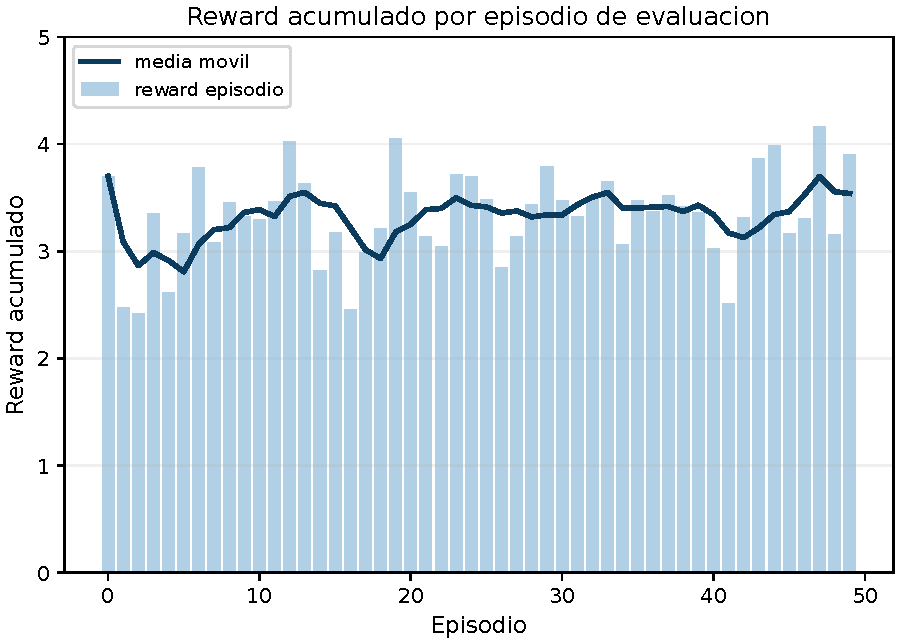
\includegraphics[width=0.47\textwidth]{figures/generated/ppo_reward_episodio.pdf}
    }
    \hfill
    \subfigure[]{
        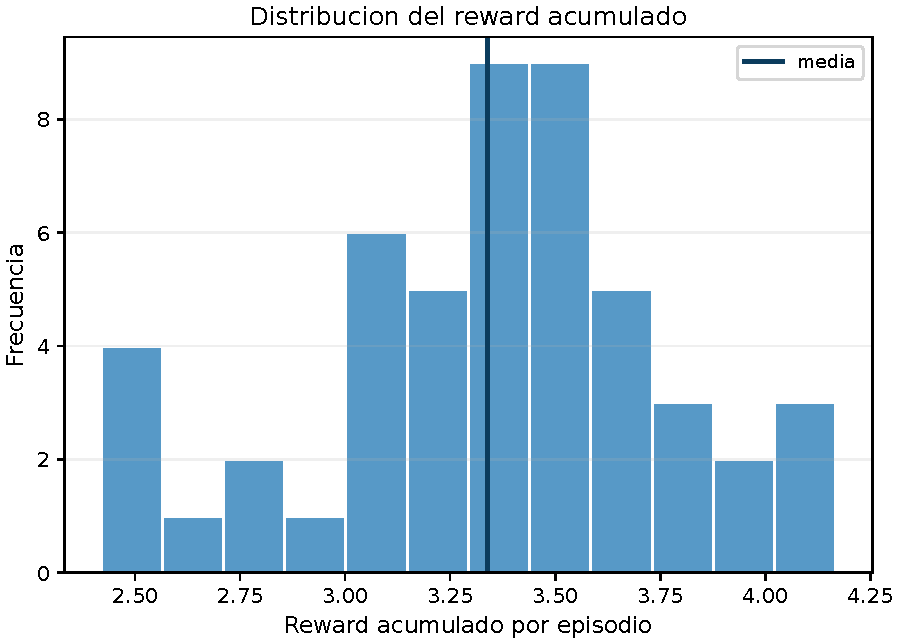
\includegraphics[width=0.47\textwidth]{figures/generated/ppo_reward_distribucion.pdf}
    }
    \caption{Resultados de reward acumulado en la evaluación PPO. La subfigura
        (a) muestra el reward total obtenido en cada episodio junto con una
        media móvil, mientras que la subfigura (b) resume la distribución del
        reward acumulado entre episodios.}
    \label{fig:ppo_reward_episodio_distribucion}
\end{figure}

La Figura~\ref{fig:ppo_reward_episodio_distribucion} resume la variabilidad del
reward acumulado durante la evaluación final. La subfigura (a) muestra el
reward total obtenido en cada episodio y una media móvil que permite observar la
tendencia sin asumir monotonía. La curva se mantiene en valores positivos,
aunque con fluctuaciones, lo cual es esperable porque cada episodio recorre una
secuencia distinta de escenarios sintéticos de drift. En particular, la demo
combina tres condiciones: \textit{covariate shift}, \textit{concept drift} y
drift combinado; cada una aparece con severidad baja, media y alta, codificada
como $0.25$, $0.60$ y $0.90$, respectivamente. Estos escenarios no representan
un único experimento fijo, sino una mezcla controlada de estados donde cambian
las señales de PSI/KS/C2ST, la caída de AUC/F1 y el costo esperado de cada
acción. Por ello, la variación entre episodios refleja que PPO enfrenta
secuencias distintas de tipo y severidad de drift, no ruido de una sola curva de
aprendizaje. La subfigura (b) muestra la distribución del reward acumulado; la
concentración alrededor de valores positivos indica que la política aprendida
tiende a obtener beneficio neto bajo la función de recompensa definida, pero
todavía conserva dispersión entre episodios.

\begin{figure}[H]
    \centering
    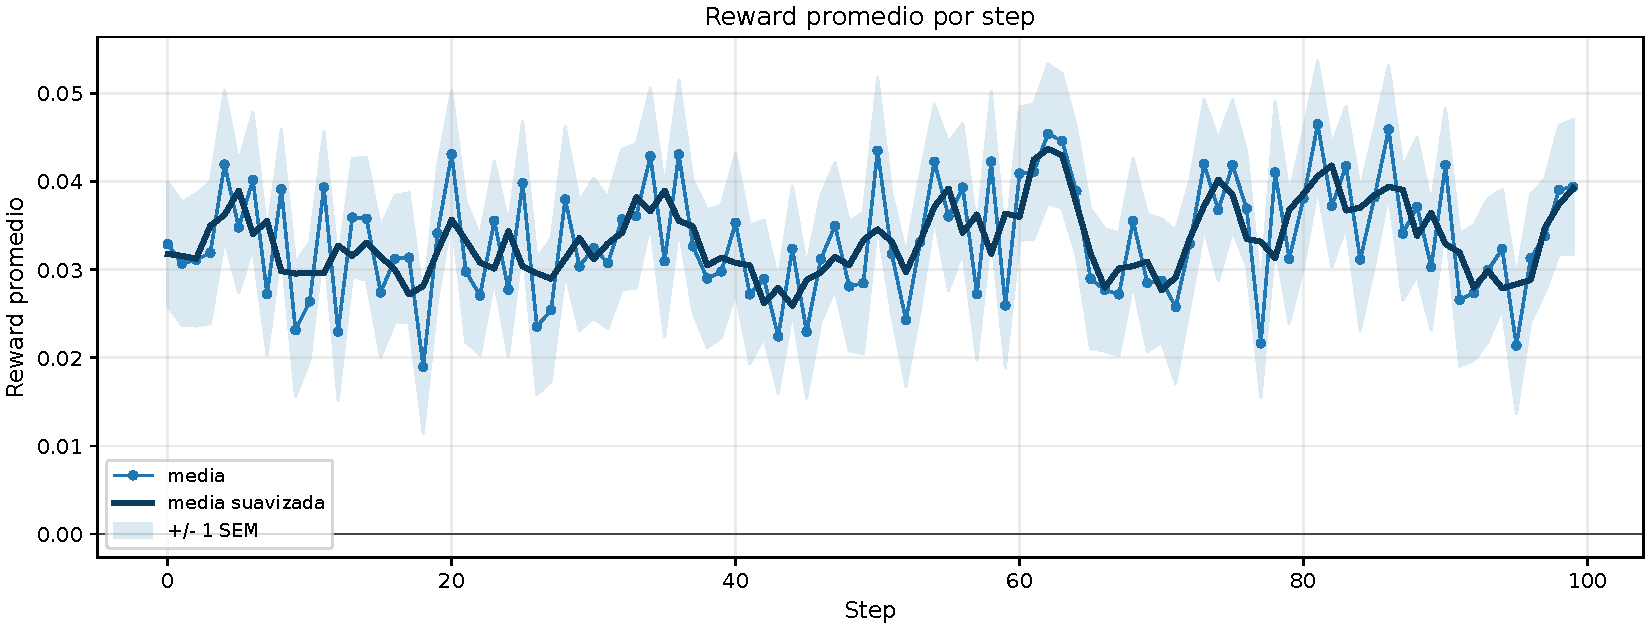
\includegraphics[width=0.98\textwidth]{figures/generated/step_reward_summary.pdf}
    \caption{Reward promedio por paso durante la evaluación PPO}
    \label{fig:ppo_reward_promedio_step}
\end{figure}

La Figura~\ref{fig:ppo_reward_promedio_step} presenta el reward promedio por
paso agregado sobre los 50 episodios. Esta gráfica representa la fase de
inferencia o evaluación determinística de una política PPO ya entrenada, no el
periodo de aprendizaje del agente. Por tanto, no debe interpretarse como una
curva de entrenamiento donde el reward necesariamente aumenta con el tiempo. En
esta demo, cada paso corresponde a un escenario de drift sintético distinto, no
a una dinámica física donde el estado deba mejorar de forma progresiva. Por
ello, las oscilaciones reflejan variabilidad entre escenarios y severidades, así
como la respuesta de la política aprendida ante cada observación. La media
suavizada y la banda de error estándar ayudan a distinguir la señal promedio del
ruido de evaluación.

\begin{figure}[H]
    \centering
    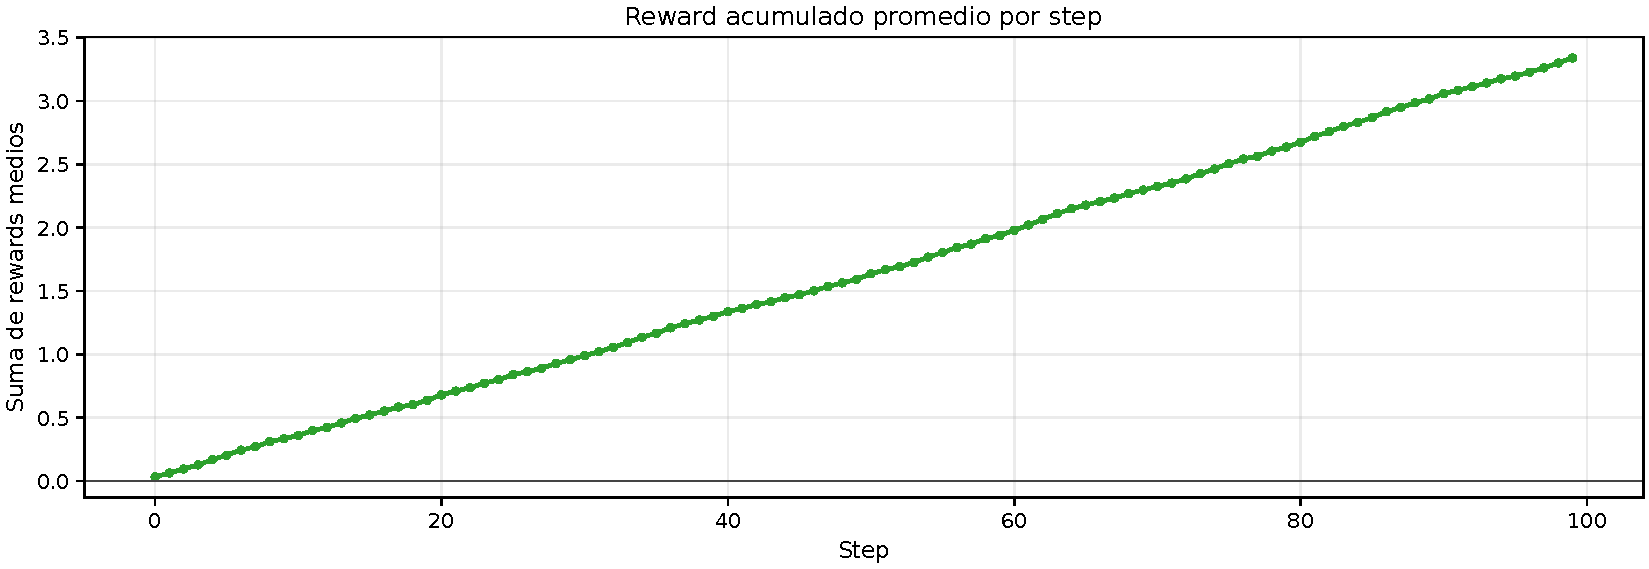
\includegraphics[width=0.98\textwidth]{figures/generated/cumulative_step_reward_summary.pdf}
    \caption{Reward acumulado promedio por paso durante la evaluación PPO}
    \label{fig:ppo_reward_acumulado_step}
\end{figure}

La Figura~\ref{fig:ppo_reward_acumulado_step} muestra la suma acumulada de los
rewards medios por paso. A diferencia del reward puntual, esta visualización
permite observar si la política conserva un beneficio agregado positivo a lo
largo del episodio. La trayectoria creciente indica que, en promedio, las
acciones seleccionadas generan más recuperación ponderada por costo que pérdida
neta. Esta evidencia es coherente con el objetivo práctico de la demo: verificar
que PPO aprende una política útil bajo observaciones parciales, sin forzar una
mejora monotónica del reward en cada paso individual.

% ------------------------------------------------------------
\section{Lectura preliminar}
% ------------------------------------------------------------

En conjunto, los resultados preliminares sugieren que la actualización selectiva
es metodológicamente plausible para DARL. La tabla empírica muestra que la
acción óptima cambia según tipo y severidad de drift, y que el costo computacional
puede cambiar la decisión incluso cuando una estrategia obtiene mayor AUC
absoluto. La demo PPO, por su parte, verifica que un agente puede aprender una
política sobre señales resumidas y seleccionar acciones parciales con reward
positivo promedio. Estos resultados no prueban todavía superioridad frente a
otros métodos, pero sí delimitan la hipótesis que debe validarse: la decisión de
mantenimiento debe depender simultáneamente del tipo de drift, la degradación de
desempeño y el costo relativo de intervenir cada etapa.

Esta lectura también justifica por qué DARL modela el \textit{pipeline} de dos
etapas como una decisión conjunta y no como dos decisiones independientes. La
etapa de preprocesamiento no produce un efecto aislado: al actualizar
\textit{features}, cambia la representación que recibe el modelo predictivo. Por
ello, una corrección de Stage 1 puede reducir señales de \textit{covariate shift},
pero también desalinear al modelo si la relación aprendida entre
variables y etiqueta no se actualiza. De forma análoga, actualizar solo Stage 2
puede ser suficiente ante señales conceptuales, pero no necesariamente corrige
una representación de entrada degradada. El contexto conjunto beneficia la
decisión porque permite evaluar cada acción por su efecto final sobre el
\textit{pipeline} completo: recuperación de AUC/F1, costo de tiempo y memoria, y
compatibilidad entre la representación producida por Stage 1 y la función
predictiva aprendida por Stage 2.

La principal limitación es que la demo PPO usa escenarios sintéticos
deterministas y livianos, diseñados para validar el flujo POMDP y no para
demostrar convergencia definitiva ni superioridad empírica. Como se desprende de
la brecha identificada en el Capítulo I, la validación completa deberá comparar
DARL contra estrategias externas y \textit{baselines} más simples: reentrenar
todo siempre, diferir siempre o aplicar umbrales simples de no acción, actualizar
solo \textit{features} con una regla fija, actualizar solo el modelo con una
regla fija, usar políticas basadas en umbrales de drift/AUC y entrenar un
clasificador supervisado que prediga una de las cuatro acciones a partir de
señales de drift, AUC/F1 y costos. Esa comparación deberá mantener la misma
definición de recuperación de AUC y costo relativo para separar qué parte del
beneficio proviene del contexto de dos etapas y qué parte proviene únicamente de
la regla de decisión usada.

\customchapter{CONCLUSIONES} 

Lorem ipsum dolor sit amet, dicant volutpat vulputate sea at. Et nam volumus voluptua, ea noster omnesque has. Qui ut graeci melius platonem. Sit fugit prompta dignissim cu. Soluta meliore repudiare vis in, eum id liber maiestatis contentiones.

\chapter*{\center \Large RECOMENDACIONES} 
\addcontentsline{toc}{section}{\bfseries RECOMENDACIONES} 
\markboth{RECOMENDACIONES}{RECOMENDACIONES} 

Lorem ipsum dolor sit amet. % sección opcional

%% ============================================================================

\renewcommand{\bibname}{\vspace{-3cm}\hfill\Large\bf{REFERENCIAS BIBLIOGRÁFICAS}\hfill}

\bibliographystyle{IEEEtran} % Estableciendo el estilo de citas IEEEtram.

\bibliography{referencias} % Recibe las referencias de IEEE

\input{secciones/anexos}

\end{document}
